% ------------------------------------------------------------------------------------------------ %
% DATA MODELING AND DATABASES
% ------------------------------------------------------------------------------------------------ %
% QUERY PROCESSING
% DATABASE INTERNALS
% REPLICATION
% SECURITY
% SQL
% CONSTRAINTS
% r1-r4 recovery
% BUSN
% ------------------------------------------------------------------------------------------------ %


\documentclass[a4paper,twocolumn]{article}


\usepackage{geometry}

% font
\usepackage{cmbright}
% no indent, but a gap between paragraphs
\usepackage{parskip}

% headings
\usepackage{titlesec}
% header and footer
\usepackage{fancyhdr}

% mathematical symbols and stuff
\usepackage{amssymb}
\usepackage{amsxtra}
% theorems
\usepackage{amsthm}

% shiny colors
\usepackage{color}
% framed boxes
\usepackage{framed}
% fancy graphics
\usepackage{tikz}

\usepackage[bf]{caption}

\usepackage{listings}

\usepackage{algorithm}
\usepackage{algorithmic}

\usepackage[pdfborder={0 0 0}]{hyperref}


% ------------------------------------------------------------------------------------------------ %


\geometry{left=10mm,right=10mm,top=25mm,bottom=25mm}
\setlength{\columnsep}{9mm}
\setlength{\parskip}{0.3em}


% ------------------------------------------------------------------------------------------------ %
% COLORS
% ------------------------------------------------------------------------------------------------ %


\definecolor{head}{rgb}{0,0,0}
\definecolor{sepline}{rgb}{0,0,0}

\definecolor{color1}{rgb}{0.10,0.30,0.80}


% ------------------------------------------------------------------------------------------------ %
% HEADINGS
% ------------------------------------------------------------------------------------------------ %


% section
\titleformat{\section}
	[display]
	{\huge\bf\raggedleft} % format
	{{\fontsize{60}{80}\selectfont\thesection}} % label
	{0pt} % sep
	{} % before
	[] % after


% ------------------------------------------------------------------------------------------------ %
% HEADER AND FOOTER
% ------------------------------------------------------------------------------------------------ %

	
\pagestyle{fancy}

% Header
\fancyhead{}
\newcommand{\activatehead}{
	\fancyhead[L]{\uppercase{Data Modeling and Databases}}
	\fancyhead[R]{\uppercase{\leftmark}}
	\renewcommand{\headrulewidth}{0.5pt}}

% Footer
\fancyfoot{}
\fancyfoot[L]{\color{head}PAGE {\thepage} / \pageref{LastPage}}
\fancyfoot[R]{\color{head}\uppercase{Jerome Dohrau}}

% Linien
\renewcommand{\headrulewidth}{0pt}
\renewcommand{\headrule}{\hrule width\headwidth height\headrulewidth \vskip-\headrulewidth}
\renewcommand{\footrulewidth}{0.5pt}
\renewcommand{\footrule}{\vskip-\footruleskip\vskip-\footrulewidth\hrule width\headwidth height\footrulewidth\vskip\footruleskip}




% ------------------------------------------------------------------------------------------------ %


\renewcommand{\phi}{\varphi}
\renewcommand{\theta}{\vartheta}

\renewcommand{\emph}[1]{\textbf{\color{color1}#1}}
\newcommand{\todo}{{\color{red}TODO}}

\newcommand{\la}{\leftarrow}
\newcommand{\ra}{\rightarrow}
\newcommand{\ramin}{\overset{\bullet}{\ra}}
\newcommand{\rara}{\ra\!\!\ra}
\newcommand{\LA}{\Leftarrow}
\newcommand{\RA}{\Rightarrow}
\newcommand{\msf}[1]{\mathsf{#1}}
\newcommand{\mbf}[1]{\mathbf{#1}}
\newcommand{\mc}[1]{\mathcal{#1}}

\renewcommand{\sp}{\;}

\newcommand{\yes}{$\surd$}
\newcommand{\no}{$\times$}

\newcommand{\join}{\mathbin{\,\tikz{
	\draw (0pt,0pt) -- (0pt,5pt);
	\draw (0pt,0pt) -- (6pt,5pt);
	\draw (0pt,5pt) -- (6pt,0pt);
	\draw (6pt,0pt) -- (6pt,5pt);}\,}}
\newcommand{\leftouterjoin}{\mathbin{\,\tikz{
	\draw (-2pt,0pt) -- (0pt,0pt) -- (0pt,5pt) -- (-2pt,5pt);
	\draw (0pt,0pt) -- (6pt,5pt);
	\draw (0pt,5pt) -- (6pt,0pt);
	\draw (6pt,0pt) -- (6pt,5pt);}\,}}
\newcommand{\rightouterjoin}{\mathbin{\,\tikz{
	\draw (0pt,0pt) -- (0pt,5pt);
	\draw (0pt,0pt) -- (6pt,5pt);
	\draw (0pt,5pt) -- (6pt,0pt);
	\draw (8pt,0pt) -- (6pt,0pt) -- (6pt,5pt) -- (8pt,5pt);}\,}}
\newcommand{\outerjoin}{\mathbin{\,\tikz{
	\draw (-2pt,0pt) -- (0pt,0pt) -- (0pt,5pt) -- (-2pt,5pt);
	\draw (0pt,0pt) -- (6pt,5pt);
	\draw (0pt,5pt) -- (6pt,0pt);
	\draw (8pt,0pt) -- (6pt,0pt) -- (6pt,5pt) -- (8pt,5pt);}\,}}
\newcommand{\leftsemijoin}{\mathbin{\,\tikz{
	\draw (0pt,0pt) -- (0pt,5pt);
	\draw (0pt,0pt) -- (6pt,5pt);
	\draw (0pt,5pt) -- (6pt,0pt);}\,}}
\newcommand{\rightsemijoin}{\mathbin{\,\tikz{
	\draw (0pt,0pt) -- (6pt,5pt);
	\draw (0pt,5pt) -- (6pt,0pt);
	\draw (6pt,0pt) -- (6pt,5pt);}\,}}


% Schusterjungen
\clubpenalty = 10000
% Hurenkinder
\widowpenalty = 10000
\displaywidowpenalty = 10000


% ------------------------------------------------------------------------------------------------ %


\newenvironment{definition}[1]
	{\textbf{#1:}}
	{}

\newenvironment{shade}
	{\definecolor{shadecolor}{rgb}{0.95,0.95,0.95}
	 \begin{shaded}}
	{\end{shaded}}

\newenvironment{note}
	{\begin{shade}\textbf{Note:}}
	{\end{shade}}

\newenvironment{example}
	{\begin{shade}\textbf{Example:}}
	{\end{shade}}

% ------------------------------------------------------------------------------------------------ %

\usetikzlibrary{shapes,shadows,arrows,decorations.pathreplacing}

\definecolor{erentity}{rgb}{1.00,0.80,0.20}
\definecolor{erattribute}{rgb}{1.00,1.00,0.40}
\definecolor{errelation}{rgb}{0.50,0.80,0.30}
\definecolor{erisa}{rgb}{0.50,0.50,1.00}

\tikzstyle{erentity}=[rectangle, draw, fill=erentity, minimum height=0.6cm, minimum width=2cm]
\tikzstyle{erweakentity}=[rectangle, draw, double distance=0.5mm, fill=erentity, minimum height=0.6cm, minimum width=2cm]
\tikzstyle{erattribute}=[ellipse, draw, fill=erattribute, minimum height=0.5cm, minimum width=1.8cm]
\tikzstyle{errelation}=[diamond, draw, fill=errelation, minimum height=1cm, minimum width=2cm]
\tikzstyle{erweakrelation}=[diamond, draw, double distance=0.5mm, fill=errelation, minimum height=1cm, minimum width=2cm]
\tikzstyle{erisa}=[regular polygon, draw, fill=erisa, regular polygon sides=6, xscale=2, minimum width=0.8cm]
\tikzstyle{area}=[draw]

\newcommand{\fsmscale}{0.75}

%drop shadow={color=gray,shadow xshift=0.05cm, shadow yshift=-0.05cm}, 
\newcommand{\fsmstate}[3]{
	\node [draw, fill=white, circle, minimum width=1.8cm,scale=\fsmscale] (#1) at (#2) {};
	\node [scale=\fsmscale]() at (#2) {\begin{tabular}{c}#3\end{tabular}};}

\newcommand{\erentity}[3]{
	\node[erentity] (#1) at (#2) {#3};}
\newcommand{\erweakentity}[3]{
	\node[erweakentity] (#1) at (#2) {#3};}
\newcommand{\erattribute}[3]{
	\node[erattribute] (#1) at (#2) {};
	\node (K) at (#2) {#3};}
\newcommand{\erattributesmall}[3]{
	\node[erattribute, minimum width=1.2cm, minimum height=0.65cm] (#1) at (#2) {};
	\node (K) at (#2) {#3};}
\newcommand{\errelation}[3]{
	\node[errelation] (#1) at (#2) {};
	\node (K) at (#2) {#3};}
\newcommand{\erweakrelation}[3]{
	\node[erweakrelation] (#1) at (#2) {};
	\node (K) at (#2) {#3};}
\newcommand{\erisa}[2]{
	\node[erisa] (#1) at (#2) {};
	\node (K) at (#2) {is-a};}


% ------------------------------------------------------------------------------------------------ %

\let\oldleftmark\leftmark

\begin{document}

% title
\twocolumn[
  \begin{@twocolumnfalse}
  \begin{center}
  {\bf\Huge{Data Modeling and Databases}}
  \end{center}
  \vspace{4em}
  {\color{sepline}\hrule}
  \vspace{2em}
  \end{@twocolumnfalse}
  ]

% table of contents
\setcounter{tocdepth}{3}
\tableofcontents
% list of figures
% \newpage
\listoffigures
\renewcommand{\leftmark}{CONTENTS}
\activatehead

\newcommand{\sectionbreak}{\clearpage}

% ------------------------------------------------------------------------------------------------ %
% INTRODUCTION
% ------------------------------------------------------------------------------------------------ %


\section{Introduction}
\renewcommand{\leftmark}{\oldleftmark}


% ------------------------------------------------------------------------------------------------ %
% MOTIVATION
% ------------------------------------------------------------------------------------------------ %


\subsection{Motivation}

A \emph{database management system} (DMBS) is used to
\begin{itemize}
\item avoid redundancy and inconsistency,
\item access the data in a declarative manner,
\item synchronize concurrent data accesses,
\item recover after a system failure,
\item guarantee security and privacy and
\item facilitate reuse of the data.
\end{itemize}


% ------------------------------------------------------------------------------------------------ %
% DATABASE ABSTRACTION LAYERS
% ------------------------------------------------------------------------------------------------ %


\subsection{Database Abstraction Layers}

\begin{figure}[htbp]
\begin{center}
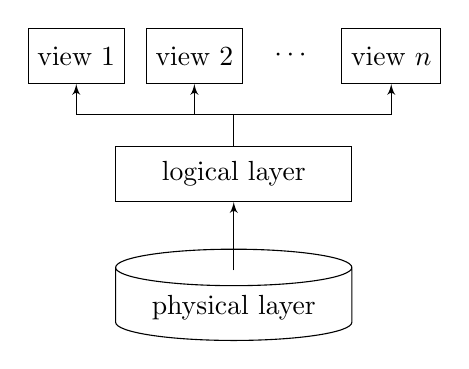
\begin{tikzpicture}[>=latex']
	\node [draw, cylinder, shape border rotate=90, aspect=0.2, minimum width=3cm] (physical) at (0cm,-0.2cm) {physical layer};
	\node [draw, rectangle, minimum width=3cm, minimum height=0.7cm] (logical) at (0cm,1.5cm) {logical layer};
	\node [draw, rectangle, minimum height=0.7cm] (view1) at (-2cm,3cm) {view 1};
	\node [draw, rectangle, minimum height=0.7cm] (view2) at (-0.5cm,3cm) {view 2};
	\node [draw, rectangle, minimum height=0.7cm] (viewn) at (2cm,3cm) {view $n$};
	\node (dots) at (0.75cm,3cm) {$\cdots$};
	\node (phantom) at (0cm,0.15cm) {};
	\path [->] (phantom) edge (logical);
	\path (logical) edge (0cm,2.25cm);
	\path [->] (-2cm,2.25cm) edge (view1);
	\path [->] (-0.5cm,2.25cm) edge (view2);
	\path [->] (2cm,2.25cm) edge (viewn);
	\path (-2cm,2.25cm) edge (2cm,2.25cm);
\end{tikzpicture}
\end{center}
\caption[Database Abstraction Layers]{The three database abstraction layers.}
\end{figure}

There are three layers of abstraction:
\begin{itemize}
\item The \emph{physical layer} determines how to store data.
\item At the \emph{logical layer} the schema of the database determines which data is stored.
\item Whereas the schema is an integrated model of the whole information, \emph{views} offer only subsets of this information.
\end{itemize}


% ------------------------------------------------------------------------------------------------ %
% DATA INDEPENDENCE
% ------------------------------------------------------------------------------------------------ %


\subsection{Data Independence}

Due to the three layers of abstraction there are two kinds of data independence:

\begin{itemize}
\item \emph{Physical data independence} is fuilfilled when modifications of the physical data structures do not affect the logical layer.
\item \emph{Logical data independence} is achieved by hiding smaller changes at the logical layer from the views.
\end{itemize}

Most of the present databases fulfill physical data independence. Logical data independence can only be guaranteed for minor modifications.


% ------------------------------------------------------------------------------------------------ %
% DATA MODELS
% ------------------------------------------------------------------------------------------------ %

\subsection{Data Modeling}

\begin{figure}[htbp]
\begin{center}
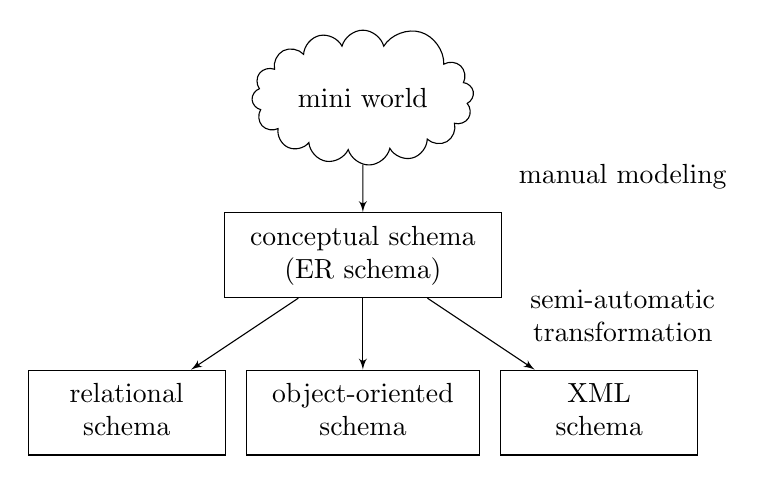
\begin{tikzpicture}[auto,>=latex']
	\node[draw, cloud, cloud puffs=15.7, aspect=2] (world) at (0cm,4cm) {mini world};
	\node[draw, rectangle] (schema) at (0cm,2cm) {\begin{tabular}{c} conceptual schema \\ (ER schema) \end{tabular}};
	\node[draw, rectangle, minimum width=2.5cm] (schema1) at (-3cm,0cm) {\begin{tabular}{c} relational \\ schema \end{tabular}};
	\node[draw, rectangle, minimum width=2.5cm] (schema2) at (0cm,0cm) {\begin{tabular}{c} object-oriented \\ schema \end{tabular}};
	\node[draw, rectangle, minimum width=2.5cm] (schema3) at (3cm,0cm) {\begin{tabular}{c} XML \\ schema \end{tabular}};
	\path [->] (world) edge (schema);
	\path [->] (schema) edge (schema1);
	\path [->] (schema) edge (schema2);
	\path [->] (schema) edge (schema3);
	\node () at (3.3cm,3cm) {manual modeling};
	\node () at (3.3cm,1.2cm) {\begin{tabular}{c} semi-automatic \\ transformation \end{tabular}};
\end{tikzpicture}
\end{center}
\caption[Data Modeling Phases]{Phases of data modeling.}
\end{figure}

There are three basic categories of models:
\begin{itemize}
\item The \emph{conceptual model} is a collection of entities and describes how they relate to each other. It captures the domain to be represented. Commonly used conceptual data models are the entity relationship model and UML.
\item The \emph{logical model} (schema) is a mapping of the concepts to a concrete logical representation. Some logical data models are the relational data model, the object-oriented data model and XML.
\item The \emph{physical model} is the implementation in a concrete hardware architecture.
\end{itemize}


% ------------------------------------------------------------------------------------------------ %
% ------------------------------------------------------------------------------------------------ %
% ENTITY RELATIONSHIP MODEL
% ------------------------------------------------------------------------------------------------ %


\section{Entity Relationship Model}

The \emph{entity relationship model} is a conceptual data model that is used to model the structure of information from the user's point of view.


% ------------------------------------------------------------------------------------------------ %


\subsection{Building Blocks of an ER Model}


% ------------------------------------------------------------------------------------------------ %
% ENTITIES AND ATTRIBUTES
% ------------------------------------------------------------------------------------------------ %


\subsubsection{Entities and Attributes}

An \emph{entity} may be defined as an object that is recognized as being capable of an independent existence and can be uniquely identified. Entities can be thought of as nouns.

Similar entities are abstracted as entity types. Entity types are graphically represented by rectangles containing the name of the entity type.

An entity is characterized by one or more \emph{attributes}. Every entity (unless it is a weak entity) must have a minimal set of uniquely identifying attributes, which is called the entity's \emph{key}. Attributes that are part of the key are underlined.

\begin{example}
In the ER model depicted in figure \ref{fig_er_model} \textit{student} and \textit{lecture} are entities. \textit{Legi} (key of student), \textit{name}, \textit{semester}, \textit{number} (key of lecture), \textit{title} and \textit{credits} are attributes.
\end{example}

\begin{figure}[htbp]
\begin{center}
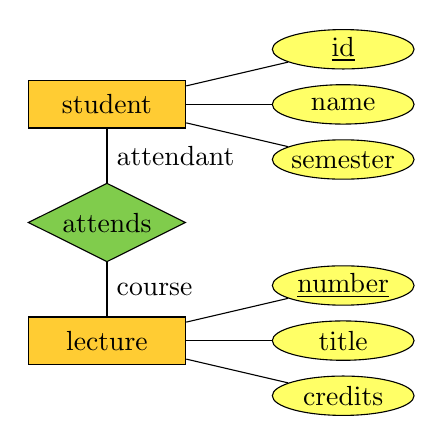
\begin{tikzpicture}[auto]
	\erentity{student}{0cm,3cm}{student}
	\erattribute{id}{3cm,3.7cm}{\underline{id}}
	\erattribute{name}{3cm,3cm}{name}
	\erattribute{semester}{3cm,2.3cm}{semester}
	
	\erentity{lecture}{0cm,0cm}{lecture}
	\erattribute{number}{3cm,0.7cm}{\underline{number}}
	\erattribute{title}{3cm,0cm}{title}
	\erattribute{credits}{3cm,-0.7cm}{credits}
	
	\errelation{attends}{0cm,1.5cm}{attends}
	
	\path (student) edge node {attendant} (attends);
	\path (student) edge (id);
	\path (student) edge (name);
	\path (student) edge (semester);
	\path (attends) edge node {course} (lecture);
	\path (lecture) edge (number);
	\path (lecture) edge (title);
	\path (lecture) edge (credits);
\end{tikzpicture}
\end{center}
\caption[Simple ER-Model]{Two related entities.}
\label{fig_er_model}
\end{figure}


% ------------------------------------------------------------------------------------------------ %
% RELATIONSHIPS AND ROLES
% ------------------------------------------------------------------------------------------------ %


\subsubsection{Relationships and Roles}

A \emph{relationship} captures how entities are related to one another and may be characterized by zero, one or more attributes. Relationships can be thought of as verbs, linking two or more nouns. They are graphically represented by a diamond shape with the name of the relationship inside.

Optionally, \emph{roles} are used to describe how an entity is involved in the relationship.

\begin{example}
In the ER model depicted in figure \ref{fig_er_model} \textit{attends} is a relationship and \textit{attendant} and \textit{course} are roles.
\end{example}


% ------------------------------------------------------------------------------------------------ %
% WEAK ENTITIES
% ------------------------------------------------------------------------------------------------ %


\subsubsection{Weak Entities}

An entity that cannot be uniquely identified by its attributes alone is called a \emph{weak entity}. To create a key it must use its attributes in conjunction with the key of an entity it is related to.

\begin{example}
Since the combination of room number and level is only unique within a building, the building's name is added to the key of room (see figure \ref{fig_weak_entity}).
\end{example}

\begin{figure}[htbp]
\begin{center}
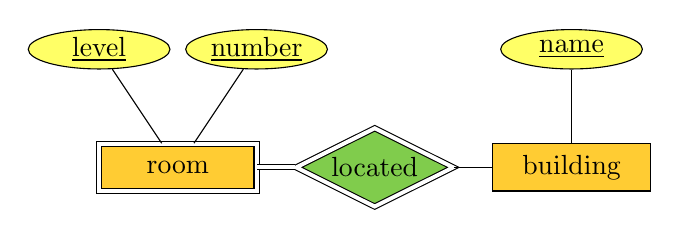
\begin{tikzpicture}[auto]
	\erweakentity{room}{0cm,0cm}{room}
	\erentity{building}{5cm,0cm}{building}
	\erweakrelation{located}{2.5cm,0cm}{located}
	
	\erattribute{level}{-1cm,1.5cm}{\underline{level}}
	\erattribute{number}{1cm,1.5cm}{\underline{number}}
	\erattribute{name}{5cm,1.5cm}{\underline{name}}
	
	\path (located) edge (building);
	\path (room) edge [double distance=0.5mm] (located);
	\path (room) edge (number);
	\path (room) edge (level);
	\path (building) edge (name);
\end{tikzpicture}
\end{center}
\caption[Weak Entity]{An example of a weak entity.}
\label{fig_weak_entity}
\end{figure}


% ------------------------------------------------------------------------------------------------ %
% CHARACTERIZATION OF A RELATIONSHIP
% ------------------------------------------------------------------------------------------------ %


\subsection{Characterization of Relationships}

A relationship $R$ between entities $E_1, E_2, \ldots, E_n$ may be considered as a relationship in the mathematical sense:
\[ \begin{array}{rcl}
R & \subseteq & E_1 \times E_2 \times \ldots \times E_n
\end{array} \]
The \emph{degree} of a relationship is given by the number of entity types $n$. In practice, most of the relationships are binary.

% \begin{note}
% The Cartesian product is defined differently from the one in set theory. The product of an $n$-tuple by an $m$-tuple is flattened into an $(n+m)$-tuple, i.e. $R \times S = \{ (r_1, \ldots, r_n, s_1, \ldots, s_m) \mid (r_1, \ldots, r_n) \in R, (s_1, \ldots, s_m) \in S$.
% \end{note}


% ------------------------------------------------------------------------------------------------ %
% CARDINALITIES OF A BINARY RELATIONSHIP
% ------------------------------------------------------------------------------------------------ %


\subsubsection{Cardinalities of Binary Relationships}

For binary relationships $R \subseteq E_1 \times E_2$ there are three basic \emph{cardinalities}:

\begin{itemize}
\item $R$ is a \emph{1:1 relationship} if for every $e_1 \in E_1$ there is at most one $e_2 \in E_2$ such that $(e_1,e_2) \in R$ and vice versa.
\item $R$ is a \emph{1:N relationship} if for every $e_2 \in E_2$ there is at most one $e_1 \in E_1$ such that $(e_1,e_2) \in R$. A single element of $E_1$ may be related to multiple elements of $E_2$.
%\item $R$ is a \emph{N:1 relationship} if for every $e_1 \in E_1$ there is at most one $e_2 \in E_2$ such that $(e_1,e_2) \in R$. A single element of $E_2$ may be related to multiple elements of $E_1$.
\item $R$ is a \emph{N:M relationship} if there are no constraints.
\end{itemize}

\begin{note}
Cardinalities are integrity constraints that need hold in the world that is modeled.
\end{note}


% ------------------------------------------------------------------------------------------------ %
% ------------------------------------------------------------------------------------------------ %


\subsubsection[Cardinalities of n-ary Relationships]{Cardinalities of $n$-ary Relationships}

The concept of cardinalities can be extended to $n$-ary relationships $R \subseteq E_1 \times E_2 \times \ldots \times E_n$. A ``$1$'' at the entity $E_k$ for some $k \in \{1,\ldots,n\}$ (like in figure \ref{fig_nary_cardinalities}) states that the relation $R$ defines a partial function
\[ \begin{array}{rclcl}
R & : & E_1 \times \ldots \times E_{k-1} \times E_{k+1} \times \ldots \times E_n & \rightarrow & E_k.
\end{array} \]

\begin{figure}[htbp]
\begin{center}
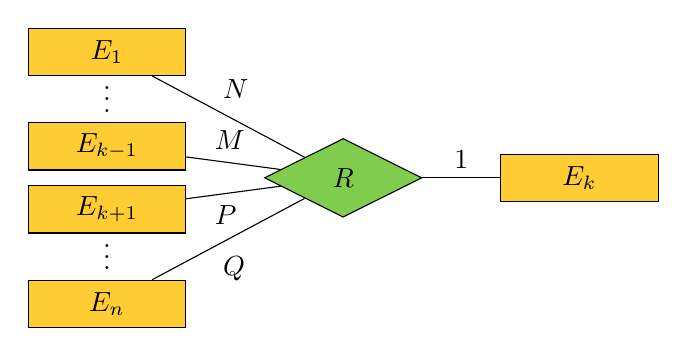
\begin{tikzpicture}[auto]
	\erentity{a}{0cm,1.6cm}{$E_1$}
	\erentity{b}{0cm,0.4cm}{$E_{k-1}$}
	\node () at (0cm,1.1cm) {$\vdots$};

	\erentity{c}{0cm,-1.6cm}{$E_{n}$}
	\erentity{d}{0cm,-0.4cm}{$E_{k+1}$}
	\node () at (0cm,-0.9cm) {$\vdots$};

	\errelation{r}{3cm,0cm}{$R$}

	\erentity{x}{6cm,0cm}{$E_k$}
	
	\path [pos=0.4] (a) edge node {$N$} (r);
	\path [pos=0.2] (b) edge node {$M$} (r);
	\path [pos=0.8] (r) edge node {$P$} (d);
	\path [pos=0.6] (r) edge node {$Q$} (c);
	\path (r) edge node {$1$} (x);
\end{tikzpicture}
\end{center}
\caption[Cardinalities of n-ary Relationships]{Cardinalities of $n$-ary relationships.}
\label{fig_nary_cardinalities}
\end{figure}


% ------------------------------------------------------------------------------------------------ %
% MIN MAX NOTATION
% ------------------------------------------------------------------------------------------------ %


\subsubsection[(min,max)-Notation]{$(min,max)$-Notation}

The \emph{$(min,max)$-notation} is another formalism to characterzie relationships:

For every entity $E_i$ of a relationship $R \subseteq E_1 \times E_2 \times \ldots \times E_n$, a pair $(min_i,max_i)$ of numbers is specified. For all $e_i  \in E_i$ at least $min_i$ records $(\ldots,e_i,\ldots)$ exist in $R$ and at most $max_i$ records $(\ldots,e_i,\ldots)$ exist in $R$. Corner cases are:
\begin{itemize}
\item If an entity need not participate in the relationship the value of $min$ is set to $0$.
\item If a single entity may participate arbitrary many times in the relationship then $max$ is replaced with $\ast$.
\end{itemize}


% ------------------------------------------------------------------------------------------------ %
% GENERALIZATION
% ------------------------------------------------------------------------------------------------ %

\subsection{Generalization}

In a conceptual model \emph{generalization} is used to obtain a more natural and well arranged structure of entities. Properties (attributes and relationships) of similar entity types are ``factorized'' and assigned to a common supertype.  Remaining properties that cannot be ``factorized'' are assigned to the respective subtype.

A subtype specializes its supertype. A supertype generalizes its subtypes. Entities (instances) of a subtype are implicitly considered as entities of the supertype too.

\begin{figure}[htbp]
\begin{center}
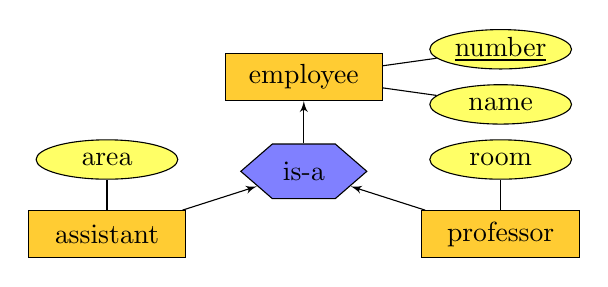
\begin{tikzpicture}[>=latex']
\erentity{employee}{0cm,2cm}{employee}
\erattribute{number}{2.5cm,2.35cm}{\underline{number}}
\erattribute{name}{2.5cm,1.65cm}{name}
\erisa{isa}{0cm,0.8cm}
\erentity{assistant}{-2.5cm,0cm}{assistant}
\erattribute{area}{-2.5cm,0.95cm}{area}
\erentity{professor}{2.5cm,0cm}{professor}
\erattribute{office}{2.5cm,0.95cm}{room}
\path (employee) edge (number);
\path (employee) edge (name);
\path [->] (isa) edge (employee);
\path [->] (assistant) edge (isa);
\path [->] (professor) edge (isa);
\path (assistant) edge (area);
\path (professor) edge (office);
\end{tikzpicture}
\end{center}
\caption[Generalization]{Generalization of employees of a university.}
\end{figure}


% ------------------------------------------------------------------------------------------------ %
% AGGREGATION
% ------------------------------------------------------------------------------------------------ %


\subsection{Aggregation}

\todo

\begin{figure}[htbp]
\begin{center}
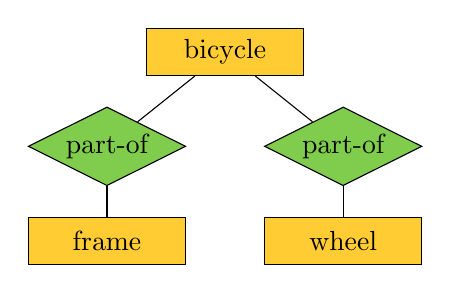
\begin{tikzpicture}
\erentity{c1}{-1.5cm,0cm}{frame}
\erentity{c2}{1.5cm,0cm}{wheel}
\errelation{partof1}{-1.5cm,1.2cm}{part-of}
\errelation{partof2}{1.5cm,1.2cm}{part-of}
\erentity{p}{0cm,2.4cm}{bicycle}
\path (c1) edge (partof1);
\path (c2) edge (partof2);
\path (p) edge (partof1);
\path (p) edge (partof2);
\end{tikzpicture}
\end{center}
\caption[Aggregation]{Parts of a bicycle.}
\end{figure}


% ------------------------------------------------------------------------------------------------ %
% CONSOLIDATION
% ------------------------------------------------------------------------------------------------ %


\subsection{Consolidation}

Often, the world to be modeled is very complex and different views are created by persons who are well versed in a part of this world. These views are generally not disjunct but need to be summarized somehow. This process is called \emph{consolidation}. The resulting schema should be consistent and without redundancy.


% ------------------------------------------------------------------------------------------------ %
% ------------------------------------------------------------------------------------------------ %
% RELATIONAL MODEL
% ------------------------------------------------------------------------------------------------ %


\section{Relational Model}

\subsection{Definition of a Relational Model}


% ------------------------------------------------------------------------------------------------ %
% MATHEMATICAL FORMALISM
% ------------------------------------------------------------------------------------------------ %


\subsubsection{Mathematical Formalism}

Let $D_1, D_2, \ldots, D_n$ be \emph{domains}. These domains may only contain atomic values (e.g. strings and integers, but no sets). A \emph{relation} $R$ is a subset of the Cartesian product of $n$ domains: 
\[ \begin{array}{rcl}
R & \subseteq & D_1 \times D_2 \times \ldots \times D_n
\end{array} \]

An element of the set $t \in R$ is called a \emph{tuple}. Since a relation is defined as a set the tuples are unordered and there are no duplicates.

\begin{note}
The domains do not need to be different, i.e. $D_i = D_j$ is possible for $i \neq j$.
\end{note}


% ------------------------------------------------------------------------------------------------ %
% DEFINITION OF A SCHEMA
% ------------------------------------------------------------------------------------------------ %


\subsubsection{Definition of a Schema}

A \emph{schema} $\mc{R}$ of a relation $R$, sometimes denoted by $\mbf{sch}(R)$, is a set of \emph{attributes} $\{A_1, \ldots, A_n\}$ that assigns a name to every component of a tuple $t \in R$.

The names of the attributes have to be unique within a relation. As in the ER model a key is a minimal set of attributes that identify each tuple uniquely.

The domain of the attribute $A_i$ is denoted by $\mbf{dom}(A_i)$. Thus, a relation $R$ is a subset of the Cartesian product of the $n$ domains $\mbf{dom}(A_1), \mbf{dom}(A_2), \ldots, \mbf{dom}(A_n)$:
\[ \begin{array}{rcl}
R & \subseteq & \mbf{dom}(A_1) \times \mbf{dom}(A_2) \times \ldots \times \mbf{dom}(A_n)
\end{array} \]


\begin{example} An address book can be modeled as a relation
\[ \begin{array}{rcl}
\msf{addressbook} & \subseteq & \msf{string \times string \times integer}.
\end{array}\]
The schema assigns names to the components of a tuple and makes the relation a lot more readable:
\[
\msf{addressbook : \{ [ name:string, address:string, \underline{tel\#:integer}] \}}
\]
The square brackets $[\ldots]$ are a tuple constructor and the curly brackets $\{\ldots\}$ indicate that the relationship is a set of tuples.
\end{example}


% ------------------------------------------------------------------------------------------------ %
% FROM AN ER MODEL TO A RELATIONAL MODEL
% ------------------------------------------------------------------------------------------------ %


\subsection{From an ER Model to a Relational Model}


% ------------------------------------------------------------------------------------------------ %
% RELATIONAL REPRESENTATION OF ENTITY TYPES
% ------------------------------------------------------------------------------------------------ %


\subsubsection[Representation of Entity Types]{Relational Representation of Entity Types}

Every attribute of the entity becomes an attribute of the relation; keys are directly adopted and stay the same.

\begin{note}
The set of attributes of a weak entity's relational representation also includes the key of the entity it depends on.
\end{note}


% ------------------------------------------------------------------------------------------------ %
% RELATIONAL REPRESENTATION OF RELATIONSHIPS
% ------------------------------------------------------------------------------------------------ %


\subsubsection[Representation of Relationships]{Relational Representation of Relationships}

The relation $R$ representing the abstract $n$-ary relationship depicted in figure \ref{fig_gen_relationship} contains all attributes of the relationship and all key attributes of the entities involved.

\[
R : \{[
\underbrace{A_{1,1}, \ldots, A_{1,k_1}}_\text{key of $E_1$}, \ldots
\underbrace{A_{n,1}, \ldots, A_{n,k_n}}_\text{key of $E_n$},
\underbrace{A_1^R, \ldots, A_{k_R}^R}_\text{attributes of $R$}
]\}
\]

\begin{figure}[htbp]
\begin{center}
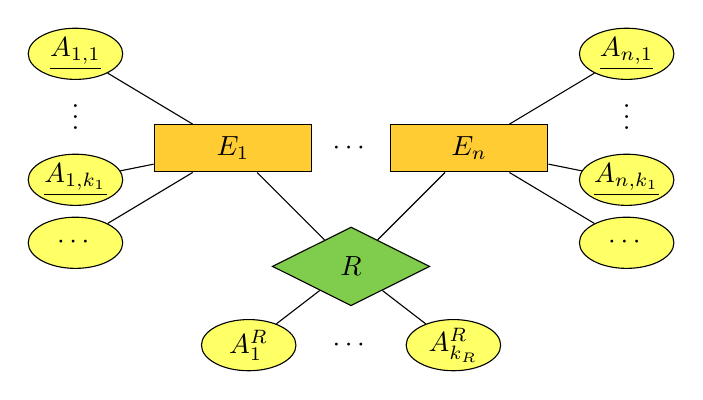
\begin{tikzpicture}

\erentity{e1}{-1.5cm,1.5cm}{$E_1$}
\erattributesmall{a11}{-3.5cm,2.7cm}{\underline{$A_{1,1}$}}
\node () at (-3.5cm,2cm){$\vdots$};
\erattributesmall{a12}{-3.5cm,1.1cm}{\underline{$A_{1,k_1}$}}
\erattributesmall{a13}{-3.5cm,0.3cm}{$\cdots$}

\node () at (0cm,1.5cm) {$\cdots$};

\erentity{en}{1.5cm,1.5cm}{$E_n$}
\erattributesmall{an1}{3.5cm,2.7cm}{\underline{$A_{n,1}$}}
\node () at (3.5cm,2cm){$\vdots$};
\erattributesmall{an2}{3.5cm,1.1cm}{\underline{$A_{n,k_1}$}}
\erattributesmall{an3}{3.5cm,0.3cm}{$\cdots$}

\errelation{r}{0cm,0cm}{$R$}
\erattributesmall{ar1}{-1.3cm,-1cm}{$A_1^R$}
\node () at (0cm,-1cm) {$\cdots$};
\erattributesmall{ark}{1.3cm,-1cm}{$A_{k_R}^R$}
\path (r) edge (e1);
\path (e1) edge (a11);
\path (e1) edge (a12);
\path (e1) edge (a13);
\path (r) edge (en);
\path (en) edge (an1);
\path (en) edge (an2);
\path (en) edge (an3);
\path (r) edge (ar1);
\path (r) edge (ark);
\end{tikzpicture}
\end{center}
\caption[n-ary Relationship]{Example of a generic $n$-ary relationship.}
\label{fig_gen_relationship}
\end{figure}

\begin{example}
The relationship depicted in figure \ref{fig_er_model} translates to:
\[
\msf{attend : \{[\underline{id:integer, number:integer}]\}}
\]
Since this is a N:M relationship \textit{id} as well as \textit{number} are part of the key.
\end{example}

In some situations relations with the same can be summarized. This works relations of 1:1 and 1:N relationships.


% ------------------------------------------------------------------------------------------------ %
% RELATIONAL ALGEBRA
% ------------------------------------------------------------------------------------------------ %


\subsection{Relational Algebra}


% ------------------------------------------------------------------------------------------------ %
% SELECTION
% ------------------------------------------------------------------------------------------------ %


\subsubsection[Selection]{Selection ($\sigma$)}

A \emph{selection} is a unary operation $\sigma_{A \circ  B}(R)$ or $\sigma_{A \circ v}(R)$, where $R$ is a relation, $A$ and $B$ are attribute names, $v$ is a constant value and $\circ \in \{=,<,\leq,>,\geq,\neq\}$ is a comparison.

The result of the selection $\sigma_{A \circ B}(R)$ contains all tuples in $R$ for which $\circ$ holds between the attributes $A$ and $B$:
\[ \begin{array}{rcl}
\sigma_{A \circ B}(R) & = & \{ t \in R \mid t.A \circ t.B \}
\end{array} \]

The result of the selection $\sigma_{A \Phi v}(R)$ contains all tuples in $R$ for which $\Phi$ holds between the attribute $A$ and the constant value $v$:
\[ \begin{array}{rcl}
\sigma_{A \Phi V}(R) & = & \{ t \in R \mid t.A \Phi v \}
\end{array} \]

A \emph{generalized selection} is a unary operation $\sigma_\phi(R)$, where $R$ is a relation and $\phi$ is a propositional formula that consists of atoms as allowed in the normal selection and the logical operators $\wedge$, $\vee$, and $\neg$. The result of this selection contains all tuples in $R$ for which $\phi$ holds:
\[ \begin{array}{rcl}
\sigma_{\phi_1 \wedge \phi_2} & = & \sigma_{\phi_1}(R) \cap \sigma_{\phi_2}(R) \\[0.5em]
\sigma_{\phi_1 \vee \phi_2} & = & \sigma_{\phi_1}(R) \cup \sigma_{\phi_2}(R) \\[0.5em]
\sigma_{\neg \phi} & = & R \setminus \sigma_{\phi}(R) 
\end{array} \]


% ------------------------------------------------------------------------------------------------ %
% PROJECTION
% ------------------------------------------------------------------------------------------------ %


\subsubsection[Projection]{Projection ($\pi$)}

The \emph{projection} operator $\pi_{A_1, \ldots, A_n}$ is defined as
\[ \begin{array}{rcl}
\pi_{A_1, \ldots, A_n}(R) & = & \{ t[A_1, \ldots, A_n] \mid t \in R \},
\end{array} \]
where $t[A_1,\ldots,A_n]$ is the tuple $t$ restricted to the attributes $A_1, \ldots, A_n$.


% ------------------------------------------------------------------------------------------------ %
% CARTESIAN PRODUCT
% ------------------------------------------------------------------------------------------------ %


\subsubsection[Cartesian Product]{Cartesian Product ($\times$)}

The  \emph{Cartesian product} $R \times S$ contains all $|R| \cdot |S|$ possible combinations of tuples in the relations $R$ and $S$:
\[ \hspace{-0.5em} \begin{array}{ll}
R \times S & = \\
\multicolumn{2}{l}{\{ [r_1,\ldots,r_n,s_1,\ldots,s_m] \mid [r_1,\ldots,r_n] \in R, [s_1,\ldots,s_m] \in S \}}
\end{array} \hspace{-0.5em} \]

\begin{note}
The Cartesian product is defined differently from the one in set theory. The Cartesian product of an $n$-tuple by an $m$-tuple is flattened into an $(n+m)$-tuple.
\end{note}

The schema of the Cartesian product $R \times S$ is
\[ \begin{array}{rclcl}
\mbf{sch}(R \times S) & = &
\mbf{sch}(R) \cup \mbf{sch}(S) & = &
\mc{R} \cup \mc{S}.
\end{array} \]
If the attribute $A$ appears in $\mc{R}$ as well as in $\mc{S}$, they are renamed as $R.A$ and $R.B$; otherwise their names would not be unique in $\mc{R} \cup \mc{S}$.


% ------------------------------------------------------------------------------------------------ %
% RENAME
% ------------------------------------------------------------------------------------------------ %


\subsubsection[Rename Operator]{Rename Operator ($\rho$)}

The operator $\rho_{R'}(R)$ \emph{renames} the relation $R$ as $R'$. And the operator $\rho_{A' \la A}$ that renames a single attribute is defined as
\[ \begin{array}{rcl}
\rho_{A' \la A}(R) & = & \{t[A' \la A] \mid t \in R\},
\end{array} \]
where $t[A' \la A]$ is the tuple $t$ with the attribute $A$ renamed as $A'$.

\begin{example} In some cases renaming is necessary. The following combination of operators returns the name of all persons and the name the persons' fathers:
\[\pi_{P_1.\msf{name},P_2.\msf{name}}(\sigma_{P_1.\msf{father}=P_2.\msf{id}}(\rho_\msf{P_1}(\msf{person}) \times \rho_\msf{P_2}(\msf{person})))\]
\end{example}


% ------------------------------------------------------------------------------------------------ %
% SET OPERATIONS
% ------------------------------------------------------------------------------------------------ %


\subsubsection[Set Operators]{Set Operators ($\cup$, $\cap$ and $\setminus$)}

Let $R$ and $S$ be two relations with the same schema (i.e. $\mc{R} = \mc{S})$. Just like in set theory, the \emph{union}, \emph{intersection} and \emph{difference} operators are
\[ \begin{array}{rcl}
R \cup S & = & \{ t \mid t \in R \vee t \in S \} \\[0.5em]
R \cap S & = & \{ t \mid t \in R \wedge t \in S \} \\[0.5em]
R \setminus S & = & \{ t \mid t \in R \wedge t \notin S \}.
\end{array} \]

% \begin{note} The intersection $R \cup S$ can be expressed by two differences:
% \[ \begin{array}{rcl}
% R \cup S & = & R \setminus (R \setminus S)
% \end{array} \]
% \end{note}


% ------------------------------------------------------------------------------------------------ %
% JOIN OPERATORS
% ------------------------------------------------------------------------------------------------ %


\subsubsection{Join Operators}
\label{join}

There is a variety of different \emph{join} operators:

\newcommand{\lefttable}{\begin{array}{|c|c|}\hline\multicolumn{2}{|c|}{R} \\\hline A & B \\\hline\hline	a_1 & b_1 \\ a_2 & b_2 \\\hline \end{array}}
\newcommand{\righttable}{\begin{array}{|c|c|} \hline\multicolumn{2}{|c|}{S} \\\hline B & C \\\hline\hline b_1 & c_1 \\ b_3 & c_2 \\\hline \end{array}}

\begin{itemize}
\item The \emph{theta join} $R \join_\theta S$, where $\theta$ is an arbitrary join predicate, can be defined as
	\[ \begin{array}{rcl}
	R \join_\theta S & = & \sigma_\theta(R \times S).
	\end{array} \]
\item The \emph{natural join} of two relations $R$ and $S$ is denoted by $R \join S$. Without loss of generality $R$ is assumed to have $n+k$ attributes $A_1,\ldots,A_n,B_1,\ldots,B_k$ and $S$ the $m+k$ attributes $B_1,\ldots,B_k,C_1,\ldots,C_m$ (where all $A_i$ and $C_j$ are pairwise different). The natural join can be defined as
	\[ \begin{array}{rcl}
	R \join S & =  & \pi_{\mc{R} \cup \mc{S}}(\sigma_\theta(R \times S)),
	\end{array} \]
	where $\theta \equiv \bigwedge_{i=1}^k R.B_i = S.B_i$.
	\[
	\begin{array}{ccccc}
	\lefttable & \join & \righttable
	& = &
	\begin{array}{|c|c|c|} \hline
	\multicolumn{3}{|c|}{R \join S} \\\hline
	A & B & C \\\hline\hline
	a_1 & b_1 & c_1 \\\hline
	\end{array}
	\end{array}
	\]
\item The \emph{left outer join} $R \leftouterjoin S$ is like the natural join, but all tuples of the left argument's relation $R$ are preserved.
	\[
	\begin{array}{ccccc}
	\lefttable & \leftouterjoin & \righttable
	& = &
	\begin{array}{|c|c|c|} \hline
	\multicolumn{3}{|c|}{R \leftouterjoin S} \\\hline
	A & B & C \\\hline\hline
	a_1 & b_1 & c_1 \\
	a_2 & b_2 & - \\\hline
	\end{array}
	\end{array}
	\]
\item The \emph{right outer join} $R \rightouterjoin S$ is analogous to the left outer join.
	\[
	\begin{array}{ccccc}
	\lefttable & \rightouterjoin & \righttable
	& = &
	\begin{array}{|c|c|c|} \hline
	\multicolumn{3}{|c|}{R \rightouterjoin S} \\\hline
	A & B & C \\\hline\hline
	a_1 & b_1 & c_1 \\
	- & b_3 & c_2 \\\hline
	\end{array}
	\end{array}
	\]
\item The \emph{outer join} $\leftouterjoin$ can be defined as
	\[ \begin{array}{rcl}
	R \outerjoin S & = & (R \leftouterjoin S) \cup (R \rightouterjoin S).
	\end{array} \]
	In this sense the outer join combines the left and right outer join.
	\[
	\begin{array}{ccccc}
	\lefttable & \outerjoin & \righttable
	& = &
	\begin{array}{|c|c|c|} \hline
	\multicolumn{3}{|c|}{R \outerjoin S} \\\hline
	A & B & C \\\hline\hline
	a_1 & b_1 & c_1 \\
	a_2 & b_2 & - \\
	- & b_3 & c_2 \\\hline
	\end{array}
	\end{array}
	\]
\item The \emph{left semi join}
	\[ \begin{array}{rcl}
	R \leftsemijoin S & = & \pi_\mc{R}(R \join S)
	\end{array} \]
	is the natural join of $R$ and $S$ projected onto the attributes of $R$.
	\[
	\begin{array}{ccccc}
	\lefttable & \leftsemijoin & \righttable
	& = &
	\begin{array}{|c|c|c|} \hline
	\multicolumn{2}{|c|}{R \leftsemijoin S} \\\hline
	A & B \\\hline\hline
	a_1 & b_1 \\\hline
	\end{array}
	\end{array}
	\]
\item The \emph{right semi join} $R \rightsemijoin S$ is analogous to the left semi join.
	\[
	\begin{array}{ccccc}
	\lefttable & \rightsemijoin & \righttable
	& = &
	\begin{array}{|c|c|c|} \hline
	\multicolumn{2}{|c|}{R \rightsemijoin S} \\\hline
	B & C \\\hline\hline
	b_1 & c_1 \\\hline
	\end{array}
	\end{array}
	\]
\end{itemize}


% ------------------------------------------------------------------------------------------------ %
% RELATIONAL DIVISION
% ------------------------------------------------------------------------------------------------ %


\subsubsection[Relational Division]{Relational Division ($\div$)}

Let $R$ and $S$ be two relations such tat $\mc{S} \subseteq \mc{R}$. The result of the \emph{relational division} $R \div S$ consists of the restrictions of tuples in $R$ to $\mc{R} \setminus \mc{S}$, for which it holds that all their combinations with tuples in $S$ are represented in $R$.

\[ \begin{array}{ccccc}
\begin{array}{|c|c|}\hline
\multicolumn{2}{|c|}{R} \\\hline
A & B \\\hline\hline
a_1 & b_1 \\
a_1 & b_2 \\
a_1 & b_3 \\
a_2 & b_2 \\
a_2 & b_3 \\\hline
\end{array}
& \div &
\begin{array}{|c|}\hline
S \\\hline
B \\\hline\hline
b_1 \\
b_2 \\\hline
\end{array}
& = &
\begin{array}{|c|}\hline
R \div S \\\hline
A \\\hline\hline
a_1 \\\hline
\end{array}
\end{array} \]

The relational division can be simulated with basic operators as follows:
\[ \begin{array}{rcl}
R \div  S & = & \pi_{\mc{R}\setminus\mc{S}}(R) \setminus \pi_{\mc{R}\setminus\mc{S}}((\pi_{\mc{R}\setminus\mc{S}}(R) \times S) \setminus R)
\end{array} \]


% ------------------------------------------------------------------------------------------------ %
% RELATIONAL CALCULUS
% ------------------------------------------------------------------------------------------------ %


\subsection{Relational Calculus}

The \emph{relational calculus} is based on the first-order predicate calculus. There are two equally powerful relational calculi:

\begin{itemize}
\item tuple relational calculus and
\item domain relational calculus.
\end{itemize}


% ------------------------------------------------------------------------------------------------ %
% TUPLE RELATIONAL CALCULUS
% ------------------------------------------------------------------------------------------------ %


\subsubsection{Tuple Relational Calculus}

Expressions in \emph{tuple relational calculus} are of the form
\[
\{ t \mid P(t) \}
\quad\text{or}\quad
\{ [t_1.A_1,\ldots,t_n.A_n \mid P(t_1,\ldots,t_n) \}
,\]
where $t,t_1,\ldots,t_n$ are tuple variable (note that $t_i=t_j$ is possible for $i\neq j$), $A_1,\ldots,A_n$ are attribute names and $P(t)$ is a predicate formula. Atoms of such a formula are
\begin{itemize}
\item $u \in R$, where $u$ is a tuple variable and $R$ is a name of a relation and
\item $u.A \circ v.B$ or $u.A \circ c$, where $u$ and $v$ are tuple variables, $A$ and $B$ attribute names, $\circ \in \{=,<,\leq,>,\geq,\neq\}$ a comparison and $c$ is a constant.
\end{itemize}

Formulae are constructed by the following rules:
\begin{itemize}
\item
	All atoms are formulae.
\item
	If $P$ is a formula, then $\neg P$ and $(P)$ are formulae too.
\item
	If $P_1$ and $P_2$ are formulae, then $P_1 \wedge P_2$, $P_1 \vee P_2$ and $P_1 \RA P_2$ are formulae too.
\item
	If $P(t)$ is a formula with a free variable $t$, then
	\[
	\forall t \in R(P(t))
	\qquad\text{and}\qquad
	\exists t \in R(P(t))
	\]
are formulae too; note that the tuple variable $t$ of the quantifications is bound to the relation $R$.
\end{itemize}

\begin{example} The expression
\[ \{
s \mid
s \in \msf{student} \wedge
\neg (\exists a \in \msf{attend}(s.\msf{id}=a.\msf{id}))
\} \]
lists all students that are attending no lectures.
\end{example}


% ------------------------------------------------------------------------------------------------ %


\subsubsection[Safe Expressions in TRC]{Safe Expressions in Tuple Relational Calculus}

Some expressions in tuple relational calculus yield infinite results. An example of such an expression is
\[ \{ t \mid \neg(t \in R) \}. \]

This is not desirable. An expression is considered \emph{safe} if its result is a subset of the domain of the formula. The domain of a formula is the set of all constants and the relations' values that appear in the formula. The result of a safe expression is always finite.


% ------------------------------------------------------------------------------------------------ %
% DOMAIN RELATIONAL CALCULUS
% ------------------------------------------------------------------------------------------------ %


\subsubsection{Domain Relational Calculus}

Expressions of \emph{domain relational calculus} are of the form
\[ \{[v_1,\ldots,v_n] \mid P(v_1,\ldots,v_n) \}, \]
where each $v_i$ (for $1 \leq i \leq n$) is a domain variable and $P(v_1,\ldots,v_n)$ denotes a predicate over the free variables $v_1,\ldots,v_n$.

Atoms of formulae in domain relational calculus are
\begin{itemize}
\item $[w_1,\ldots,w_m] \in R$, where $R$ is an $m$-ary relation and
\item $x \circ y$ and $x \circ c$, where $x$ and $y$ are domain variables, $c$ is a constant and $\circ \in \{=,<,\leq,>,\geq,\neq\}$ is a comparison.
\end{itemize}

Formulae are constructed according to the following rules:
\begin{itemize}
\item
	An atom is a formula.
\item
	If $P$ is a formula, then $\neg P$ and $(P)$ are formulae too.
\item
	If $P_1$ and $P_2$ are formulae, then $P_1 \wedge P_2$, $P_1 \vee P_2$ and $P_1 \RA P_2$ are formulae too.
\item
	If $P(v)$ is a formula with a free variable $t$, then
	\[ \forall v (P(v))
	\qquad\text{and}\qquad
	\exists v (P(v)) \]
	are formulae too.
\end{itemize}

\begin{example}
The expression
\[ \begin{array}{rcl} \{
[i,n] & \mid & \exists s ([i,n,s] \in \msf{student} \\
& \wedge & \exists n' ([i,n'] \in \msf{attends} \\
& \wedge & \exists t,c ([n',t,c] \in \msf{lecture} \\
& \wedge & c \geq 8 ))) \}
\end{array} \]
lists the id and name of all students that attend a lecture with more at least $8$ credits (compare with ER model in figure \ref{fig_er_model}).
\end{example}


% ------------------------------------------------------------------------------------------------ %
% SAFE EXPRESSIONS IN DOMAIN RELATIONAL CALCULUS
% ------------------------------------------------------------------------------------------------ %


\subsubsection[Safe Expressions in DRC]{Safe Expressions in Domain Relational Calculus}

Like in the tuple relational calculus the domain relational calculus allows infinite results:
\[
\{ [v_1,\ldots,v_n] \mid \neg([v_1,\ldots,v_n] \in R) \}
\]

An expression $\{[v_1,\ldots,v_n\mid P(v_1,\ldots,v_n)\}$ is \emph{safe}, if the following conditions hold:
\begin{itemize}
\item If the tuple $[v_1,\ldots,v_{i-1},c_i,v_{i+1},\ldots,v_n]$, where $c_i$ is a constant, is contained in the result, then $c_i$ must be contained in the domain of $P$.
\item Every existentially quantified subformula $\exists v(P'(v))$ may only accept elements of the domain of $P'$. In other words: If $P'(c)$ holds for a constant value, then $c$ is contained in the domain of $P'$.
\item Every universally quantified subformula $\forall v(P'(v))$ holds, if and only if $P'(v)$ holds for every value in the domain of $P'$. In other words: $P'(c)$ holds for all values $c$ that are not contained in the domain of $P'$.
\end{itemize}


% ------------------------------------------------------------------------------------------------ %
% CODD'S THEOREM
% ------------------------------------------------------------------------------------------------ %


\subsection{Codd's Theorem}

\emph{Codd's theorem} states that
\begin{itemize}
\item relational algebra,
\item tuple relational calculus restricted to safe expressions and
\item domain relational calculus restricted to safe expressions
\end{itemize}
are precisely equivalent in expressive power. That is, a database query can be formulated in one language if and only if it can be expressed in the others.

Query languages that are equivalent in expressive power to relational algebra are called \emph{relationally complete}.


% ------------------------------------------------------------------------------------------------ %
% ------------------------------------------------------------------------------------------------ %
% RELATIONAL DESIGN THEORY
% ------------------------------------------------------------------------------------------------ %


\section{Relational Design Theory}


% ------------------------------------------------------------------------------------------------ %
% FUNCTIONAL DEPENDENCIES
% ------------------------------------------------------------------------------------------------ %


\subsection{Functional Dependencies}

A \emph{functional dependency (FD)} is a constraint between two sets of attributes in a relation of a database.

Let $\mc{R}$ be the schema of a relation $R$. A set of attributes \mbox{$\alpha \subseteq \mc{R}$} is said to functionally determine another set of attributes $\beta \subseteq \mc{R}$, if and only if
\[ \begin{array}{cccc}
\forall r,t \in R: &
r.\alpha = t.\alpha
& \RA &
r.\beta = t.\beta.
\end{array}\]
Such a functional dependency is denoted by
\[ \alpha \ra \beta \]

\begin{note}
 $XY \ra Z$ is a sloppy notation for $\{X,Y\}\ra\{Z\}$.
\end{note}

A functional dependency $\alpha \ra \beta$ is \emph{minimal}, written \mbox{$\alpha \ramin \beta$}, if and only if
\[ \begin{array}{cc}
\forall A \in \alpha: & \alpha\setminus\{A\} \not\ra \beta.
\end{array} \]

A functional dependency $\alpha \ra \beta$ is \emph{trivial}, if $\beta \subseteq \alpha$.


% ------------------------------------------------------------------------------------------------ %
% ARMSTRONG'S AXIOMS AND CONCLUSIONS
% ------------------------------------------------------------------------------------------------ %


\subsubsection{Armstrong's Axioms and Conclusions}
\label{armstrongs_axioms}

The three \emph{Armstrong's axioms} are used to infer all the functional dependencies:
\begin{itemize}
\item \emph{Reflexivity:} $\beta \subseteq \alpha \RA \alpha \ra \beta$
\item \emph{Augmentation:} $\alpha \ra \beta \RA \alpha\gamma \ra \beta\gamma$
\item \emph{Transitivity:} $\alpha \ra \beta \wedge \beta \ra \gamma \RA \alpha \ra \gamma$
\end{itemize}

The Armstrong axioms are sound and complete. Some other rules that can be concluded from these axioms are:
\begin{itemize}
\item \emph{Union rule:} $\alpha \ra \beta \wedge \alpha \ra \gamma \RA \alpha \ra \beta\gamma$
\item \emph{Decomposition:} $\alpha \ra \beta\gamma \RA \alpha \ra \beta \wedge \alpha \ra \gamma$
\item \emph{Pseudo transitivity:} $\alpha \ra \beta \wedge \beta\gamma \ra \delta \RA \alpha\gamma \ra \delta$
\end{itemize}

\begin{note}
The closure $F^+$ of a set of functional dependencies $F$ contains all functional dependencies that can be inferred from $F$, using the rules described above.
\end{note}


% ------------------------------------------------------------------------------------------------ %


\subsubsection{Closure of Attributes}

The \emph{closure} of a set of attributes $\alpha$, denoted by $\alpha^+$, is the largest set of attributes that is functionally determined by $\alpha$.

The following algorithm takes a set of functional dependencies $F$ and a set of attributes $\alpha$ as input and computes the closure $\alpha^+$ such that $\alpha \ra \alpha^+$:

\begin{algorithm}
\caption*{\bf AttrClosure($F$,$\alpha$)}
\begin{algorithmic}
\STATE{$\alpha^+ := \alpha$}
\WHILE{$\alpha^+$ has changed}
	\FORALL{$\beta \ra \gamma \in F$}
		\IF{$\beta \subseteq \alpha^+$}
			\STATE{$\alpha^+ := \alpha^+ \cup \gamma$}
		\ENDIF
	\ENDFOR
\ENDWHILE
\RETURN{$\alpha^+$}
\end{algorithmic}
\end{algorithm}


% ------------------------------------------------------------------------------------------------ %
% MINIMAL BASIS
% ------------------------------------------------------------------------------------------------ %


\subsubsection{Minimal Basis}

Two set $F$ and $G$ of functional dependencies are equivalent, denoted by $F \equiv G$, if and only if their closures are the same, i.e. $F^+ = G^+$.

$F_c$ is called \emph{minimal basis} of $F$ if and only if:
\begin{enumerate}
\item $F_c \equiv F$, i.e. the closure of $F_c$ and $F$ are the same.
\item There is no functional dependency $\alpha \ra \beta \in F_c$ that contains unnecessary attributes:
	\begin{enumerate}
	\item $\forall A \in \alpha : F_c \not\equiv F_c \setminus (\alpha \ra \beta) \cup ((\alpha \setminus \{A\}) \ra \beta)$
	\item $\forall B \in \beta : F_c \not\equiv F_c \setminus (\alpha \ra \beta) \cup (\alpha \ra (\beta \setminus \{ B \}))$
	\end{enumerate}
\item There are no two functional dependencies in $F_c$ with the same left side. This can be achieved by applying the union rule.
\end{enumerate}

Given a set of functional dependencies $F$ the minimal basis $F_c$ of $F$ is computed as follows:
\begin{enumerate}
\item
	For every $\alpha \ra \beta \in F$ perform a reduction of the left side; i.e. if for an $A \in \alpha$ the condition
	\[ \beta \subseteq \msf{AttrClosure}(F,\alpha \setminus \{A\}) \]
	holds, then replace $\alpha \ra \beta$ with $(\alpha\setminus\{A\})\ra\beta$.
\item
	For every remaining $\alpha \ra \beta \in F$ perform a reduction of the right side; i.e. if for a $B \in \beta$ the condition
	\[ B \in \msf{AttrClosure}(F\setminus(\alpha\ra\beta)\cup(\alpha\ra(\beta\setminus\{B\})),\alpha) \]
	holds, then replace $\alpha \ra \beta$ with $\alpha \ra (\beta\setminus\{B\})$.
\item Remove all functional dependencies of the form $\alpha \ra \emptyset$.
\item If there are functional dependencies with the same right side $\alpha \ra \beta_1, \ldots, \alpha \ra \beta_n$, apply the union rule to replace them with a single functional dependency \mbox{$\alpha \ra \cup_{i=1}^n \beta _i$}.
\end{enumerate}


% ------------------------------------------------------------------------------------------------ %
% MULTIVALUE DEPENDENCIES
% ------------------------------------------------------------------------------------------------ %


\subsection{Multivalued Dependencies}

Let $\mc{R}$ be the schema of a relation $R$. Furthermore let $\alpha \subseteq \mc{R}$ and $\beta \subseteq \mc{R}$ be two subsets of $\mc{R}$ and $\gamma = \mc{R} \setminus (\alpha \cup \beta)$. The \emph{multivalued dependency (MVD)}
\[ \alpha \rara \beta \]
holds, if and only if for all pairs of tuples $t_1$ and $t_2$ in $R$ with $t_1.\alpha = t_2.\alpha$, there exist tuples $t_3$ and $t_4$ in $R$ such that
\[ \begin{array}{rcrclcl}
t_1.\alpha & = & t_2.\alpha & = & t_3.\alpha & = & t_4.\alpha \\
& & t_3.\beta  & = & t_2.\beta  & & \\
& & t_3.\gamma & = & t_1.\gamma & & \\
& & t_4.\beta  & = & t_1.\beta  & & \\
& & t_4.\gamma & = & t_2.\gamma. & & \\
\end{array} \]

In other words: If there are two tuples with the same $\alpha$-values, their $\beta$-values can be swapped and the resulting tuples have to exist in the relation.

\begin{example} In the following relation $R$, the multivalued dependencies $A \rara B$ and $A \rara C$ hold:
\[ \begin{array}{|c|c|c|}\hline
\multicolumn{3}{|c|}{R} \\\hline
A & B & C \\\hline\hline
a_1 & b_1 & c_1 \\
a_1 & b_2 & c_2 \\
a_1 & b_2 & c_1 \\
a_1 & b_1 & c_2 \\\hline
\end{array} \]
\vspace*{-1em}
\end{example}

A multivalued dependency $\alpha \rara \beta$ is \emph{trivial}, if and only if $\beta\subseteq\alpha$ or $\beta = \mc{R}\setminus\alpha$.


% ------------------------------------------------------------------------------------------------ %
% PROPERTIES OF MULTIVALUED DEPENDENCIES
% ------------------------------------------------------------------------------------------------ %


\subsubsection[Properties of MVD]{Properties of Multivalued Dependencies}

Some rules for multivalued dependencies are:
\begin{itemize}
\item \emph{Complement:} $\alpha \rara \beta \RA \alpha \rara \mc{R}\setminus (\alpha \cup \beta)$
\item \emph{M.v. augmentation:}	$\alpha\rara\beta \wedge \delta\subseteq\gamma \RA \alpha\gamma \rara \beta\delta$
\item \emph{M.v. transitivity:} $\alpha\rara\beta \wedge \beta\rara\gamma \RA \alpha\rara\gamma\setminus\beta$
\item \emph{Generalization:} $\alpha\ra\beta \RA \alpha\rara\beta$
\item \emph{Coalesce:} $\alpha\rara\beta \wedge \gamma\subseteq\beta \wedge \delta\cup\beta=\emptyset \wedge \delta\ra\gamma \RA \alpha\ra \gamma$
\item \emph{M.v. union:} $\alpha\rara\beta \wedge \alpha \rara\gamma \RA \alpha \rara \beta\gamma$
\item \emph{Intersection:} $\alpha\rara\beta \wedge \alpha\rara\gamma \RA \alpha \rara \beta \cap \gamma$
\item \emph{Difference:} $\alpha\rara\beta \wedge \alpha\rara\gamma \RA \alpha\rara\beta\setminus\gamma$
\end{itemize}

\begin{note}
The closure $D^+$ of a set of functional and multivalues dependencies $D$ contains all dependencies that can be derived from $D$, using the rules described above and in section \ref{armstrongs_axioms}.
\end{note}


% ------------------------------------------------------------------------------------------------ %
% KEYS
% ------------------------------------------------------------------------------------------------ %


\subsection{Keys}

Let $\mc{R}$ be the schema of a relation $R$. A set of attributes $\alpha \subseteq \mc{R}$ is a \emph{superkey}, if and only if
\[
\alpha \ra \mc{R}.
\]
I.e. determines all other attributes in $\mc{R}$. If $\alpha \ramin \mc{R}$ holds, then $\alpha$ is called a \emph{candidate key} of $\mc{R}$.

\begin{note} In order to check whether $\kappa$ is a superkey of $\mc{R}$ with respect to the functional dependencies $F$, the closure \mbox{$\kappa^+ = \msf{AttrClosure}(F,\kappa)$} is determined. $\kappa$ is a superkey if $\kappa^+ = \mc{R}$.
\end{note}


% ------------------------------------------------------------------------------------------------ %
% BAD RELATINAL SCHEMAS
% ------------------------------------------------------------------------------------------------ %


\subsection{Bad Relational Schemas}

Badly designed schemas may lead to \emph{anomalies}. There are three kinds of anomalies:
\begin{itemize}
\item \emph{Update anomaly:} Redundancy may lead to inconsistency when data is updated. This is also a place complexity and performance issue.
\item \emph{Insert anomaly:} \todo
\item \emph{Delete anomaly:} \todo
\end{itemize}


% ------------------------------------------------------------------------------------------------ %
% DECOMPOSITION OF RELATIONS
% ------------------------------------------------------------------------------------------------ %


\subsection{Decomposition of Relations}

A set of schemas $\{ \mc{R}_1,\mc{R}_2,\ldots,\mc{R}_n \}$ is a \emph{decomposition} of a schema $\mc{R}$, if all attributes are preserved, i.e.
\[ \begin{array}{rcl}
\mc{R} & = & \mc{R}_1 \cup \mc{R}_2 \cup \ldots \cup \mc{R}_n.
\end{array} \]

The corresponding decomposition of a relation $R$ into the set of relations $\{R_1,R_2,\ldots,R_n\}$ is defined as
\[ \begin{array}{ccc}
 R_i & := & \pi_{\mc{R}_i}(R) \qquad\text{for $1\leq i \leq n$.}
\end{array} \]

% ------------------------------------------------------------------------------------------------ %
% LOSSLESS DECOMPOSITIONS
% ------------------------------------------------------------------------------------------------ %


\subsubsection{Lossless Decompositions}

A decomposition of $\mc{R}$ into $\mc{R}_1$ and $\mc{R}_2$ is \emph{lossless}, if
\[ \begin{array}{rcl}
R & = & R_1 \join R_2
\end{array} \]
holds for every instance $R$ of $\mc{R}$.

A decomposition of $\mc{R}$ with functional dependencies $F_\mc{R}$ into $\mc{R}_1$ and $\mc{R}_2$ is lossless, if it is possible to infer
\[ (\mc{R}_1\cap\mc{R}_2) \ra \mc{R}_1 \in F_\mc{R}^+
\quad\text{or}\quad
(\mc{R}_1\cap\mc{R}_2) \ra \mc{R}_2 \in F_\mc{R}^+. \]

\begin{note}
This is a sufficient, but not a necessary condition.
\end{note}


% ------------------------------------------------------------------------------------------------ %
% PRESERVATION OF FUNCTIONAL DEPENDENCIES
% ------------------------------------------------------------------------------------------------ %


\subsubsection{Preservation of Dependencies}

The decomposition $\{\mc{R}_1,\mc{R}_2,\ldots,\mc{R}_n\}$ of $\mc{R}$ with functional dependencies $F_\mc{R}$ is \emph{dependency preserving} if
\[ \begin{array}{rcl}
F_\mc{R} & \equiv & (F_{\mc{R}_1} \cup F_{\mc{R}_2} \cup \ldots \cup F_{\mc{R}_n}),
\end{array} \]
where $F_{\mc{R}_i} = \{ \alpha\ra\beta \in F_\mc{R}^+ \mid \alpha \cup \beta \subseteq \mc{R}_i \}$ for $1 \leq i \leq n$.

\todo


% ------------------------------------------------------------------------------------------------ %
% NORMAL FORMS
% ------------------------------------------------------------------------------------------------ %


\subsection{Normal Forms}


% ------------------------------------------------------------------------------------------------ %
% FIRST NORMAL FORM
% ------------------------------------------------------------------------------------------------ %


\subsubsection{First Normal Form}

The \emph{first normal form (1NF)} requires that domains contain only atomic values. This holds due to the definition of the relational model.


% ------------------------------------------------------------------------------------------------ %
% SECOND NORMAL FORM
% ------------------------------------------------------------------------------------------------ %


\subsubsection{Second Normal Form}

Let $\kappa_1, \kappa_2, \ldots, \kappa_n$ be the candidate keys of the schema $\mc{R}$ with functional dependencies $F$. The schema $\mc{R}$ is in \emph{second normal form (2NF)}, if and only if
\[ \kappa_i \ramin A \in F^+ \]
holds for every $1 \leq i \leq n$ and $A \in \mc{R}\setminus\{\kappa_1\cup\kappa_2\cup\ldots\cup\kappa_n)$. I.e. every non key attribute is minimally dependent on every key.

\begin{note}
2NF implies 1NF
\end{note}


% ------------------------------------------------------------------------------------------------ %
% THIRD NORMAL FORM
% ------------------------------------------------------------------------------------------------ %


\subsubsection{Third Normal Form}

A schema $\mc{R}$ is in \emph{third normal form (3NF)}, if for every functional dependency of the form $\alpha \ra A$, with $\alpha \subseteq \mc{R}$ and $A \in \mc{R}$, at least on of the following conditions holds:
\begin{itemize}
\item $A \in \alpha$, i.e. the functional dependency is trivial.
\item The attribute $A$ is contained in a candidate key of $\mc{R}$.
\item $\alpha$ is a superkey of $\mc{R}$.
\end{itemize}

\begin{note}
3NF implies 2NF.
%The third normal form implies the second normal form.
\end{note}

The following \emph{synthesis algorithm} takes a schema $\mc{R}$ and a set of functional dependencies $F$ as input and computes a lossless and dependency preserving decomposition $\{\mc{R}_1,\ldots,\mc{R}_n\}$ of $\mc{R}$, such that every $\mc{R}_i$ is in 3NF:
\begin{enumerate}
\item
	Compute the minimal basis $F_c$ of $F$.
\item
	For every $\alpha \ra \beta \in F_c$:
	\begin{enumerate}
	\item Create a relational schema $\mc{R}_\alpha := \alpha \cup \beta$
	\item Define $F_\alpha := \{ \alpha' \ra \beta' \in F_c \mid \alpha' \cup \beta' \subseteq \mc{R}_\alpha \}$ to be the functional dependencies of $\mc{R}_\alpha$.
	\end{enumerate}
\item
	If none of the schemas $\mc{R}_\alpha$ contains a candidate key of $\mc{R}$ with respect to $F_c$: Choose a candidate key $\kappa \subseteq \mc{R}$ and define the schema $\mc{R}_\kappa$ with $F_\kappa := \emptyset$.
\item
	Eliminate all schemas $\mc{R}_\alpha$ that are contained in another schema $\mc{R}_{\alpha'}$ (i.e. $\mc{R}_\alpha \subseteq \mc{R}_{\alpha'}$).
\end{enumerate}


% ------------------------------------------------------------------------------------------------ %
% BOYCE-CODD NORMAL FORM
% ------------------------------------------------------------------------------------------------ %


\subsubsection{Boyce-Codd Normal Form}
\label{bcnf}

A schema $\mc{R}$ is in \emph{Boyce-Codd normal form (BCNF)}, if for every functional dependency $\alpha \ra \beta$, at least one of the following two conditions holds:
\begin{itemize}
\item $\beta \subseteq \alpha$, i.e. the functional dependency is trivial.
\item $\alpha$ is a superkey of $\mc{R}$.
\end{itemize}

The following \emph{decomposition algorithm} takes a schema $\mc{R}$ as input and computes a lossless decomposition $\{\mc{R}_1,\ldots,\mc{R}_n\}$, such that every $\mc{R}_i$ is in BCNF:

\begin{enumerate}
\item
	Start with $Z = \{ \mc{R} \}$.
\item
	While there is a schema $\mc{R}_i \in Z$, that is not in BCNF:
	\begin{enumerate}
	\item Find a non-trivial functional dependency $\alpha \ra \beta$ for $\mc{R}_i$, such that $\alpha \cap \beta = \emptyset$ and $\alpha \not\ra \mc{R}_i$.
	\item Decompose $\mc{R}_i$ into $\mc{R}_{i_1} := \alpha \cup \beta$ and $\mc{R}_{i_2} := \mc{R}_i \setminus \beta$.
	\item Update $Z := (Z \setminus \mc{R}_i) \cup \{ \mc{R}_{i_1}, \mc{R}_{i_2} \}$.
	\end{enumerate}
\end{enumerate}

\begin{note}
The decomposition computed by this algorithm is in general not dependency preserving.
\end{note}

\begin{note}
BCNF implies 3NF
\end{note}

% ------------------------------------------------------------------------------------------------ %
% FOURTH NORMAL FORM
% ------------------------------------------------------------------------------------------------ %


\subsubsection{Fourth Normal Form}

A schema $\mc{R}$ with the set of dependencies $D$ is in \emph{fourth normal form (4NF)}, if and only if for all $\alpha \rara \beta \in D^+$ at least one of the following conditions holds:
\begin{itemize}
\item $\alpha \rara \beta$ is trivial, i.e $\beta \subseteq \alpha$ or $\beta = \mc{R}\setminus\alpha$.
\item $\alpha$ is a superkey of $\mc{R}$.
\end{itemize}

\begin{note}
4NF implies BCNF.
\end{note}

The decomposition algorithm for 4NF is analogous to the one for BCNF described in section \ref{bcnf}.


% ------------------------------------------------------------------------------------------------ %
% ------------------------------------------------------------------------------------------------ %
% DATABASE INTERNALS
% ------------------------------------------------------------------------------------------------ %


\section{Database Internals}


% ------------------------------------------------------------------------------------------------ %
% DATABASE OPTIMIZATIONS
% ------------------------------------------------------------------------------------------------ %


\subsection{Database Optimizations}

% \begin{itemize}
% \item The \emph{query processor} uses efficient algorithms for SQL operators and optimizes the database by ordering the operators, semanticly rewritings the queries and parallel execution.
% \item The \emph{storage manager} is responsible for the layout of the data on the backend storage, manages the buffer and caches and enforces load and admission control.
% \end{itemize}

Many DBMS tasks, like load control and buffer management, are also carried out by the operating system. However the database has intimate knowledge of the workload an can predict the pattern of a query. In contrast, the operating system does generic optimizations. Sometimes the operating system overrides DBMS optimizations.


% ------------------------------------------------------------------------------------------------ %
% STORAGE HIERARCHY
% ------------------------------------------------------------------------------------------------ %


\subsection{Storage Hierarchy}


The storage of a database is organized in a hierarchy; different media ar combined to mimic one ideal storage. Higher layers of the hierarchy \textit{buffer} data of lower layers by exploiting spatial and temporal locality of applications.

Furthermore the storage system can be distributed.



% ------------------------------------------------------------------------------------------------ %
% BUFFER MANAGEMENT
% ------------------------------------------------------------------------------------------------ %


\subsection{Buffer Management}

A \emph{buffer} is used to minimize disk accesses; pages are kept in main memory as long as possible. The buffer \emph{replacement policy} defines which frame is chosen for replacement. Depending on the \emph{access pattern} (sequential, hierarchical, random, cyclic) the policy can have a big impact on the number of I/O operations.

A page that is requested many times can be pinned by increasing the \emph{pin count}. A page is a candidate for replacement if it is unpinned, i.e. the pin count is zero.



% ------------------------------------------------------------------------------------------------ %
% LEAST RECENTLY USED POLICY
% ------------------------------------------------------------------------------------------------ %


\subsubsection{Least Recently Used}

For each page in the puffer pool, the time of the last unpinning is kept track of. The \emph{least recently used (LRU)} policy replaces the page with the oldest time.

\begin{note}
However, for sequential flooding ($1,2,\ldots,n,1,2,\ldots$) the most recently used policy works better.
\end{note}


% ------------------------------------------------------------------------------------------------ %
% CLOCK REPLACEMENT
% ------------------------------------------------------------------------------------------------ %


\subsubsection{Clock Replacement}

The \emph{clock replacement} policy is an approximation of LRU. It arrenges the frames into a cycle and stores a \emph{reference bit} per page (One can think of this as a second chance bit). When the pin count of a page is reduced to zero, the reference bit is turned on.

When a replacement is necessary, the policy loops through the pages in the cycle and
\begin{itemize}
\item if the pin count of the page is zero and the reference bit is on, the reference bit is turned off and
\item if the pincount is zero and the reference bit is off, the page is chosen for replacement.
\end{itemize}



% ------------------------------------------------------------------------------------------------ %
% DATA MANAGER
% ------------------------------------------------------------------------------------------------ %


\subsection{Data Manager}

\todo


% ------------------------------------------------------------------------------------------------ %
% ------------------------------------------------------------------------------------------------ %
% QUERY PROCESSING
% ------------------------------------------------------------------------------------------------ %


\subsection{Query Processing}


There are three approaches to process a query:
\begin{itemize}
\item Compile a query into machine code. This approach achieves high performance.
\item Compile a query into relational algebra and interpret the resulting expression. This is easier to debung and has better portability.
\item Use a hybrid solution.
\end{itemize}

\begin{figure}[htbp]
\begin{center}
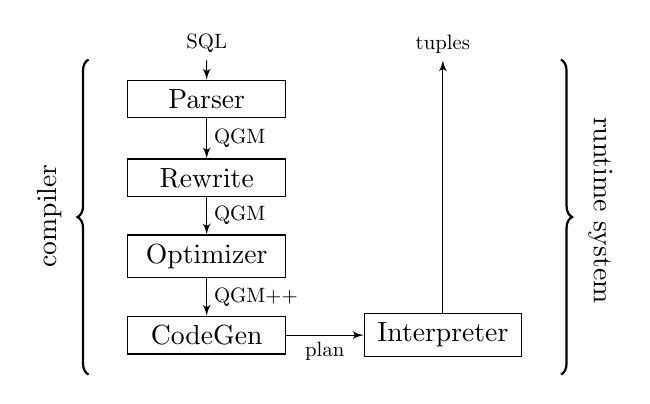
\begin{tikzpicture}[auto,>=latex']
	\node [scale=0.75] (n0) at (0cm,3.7cm) {SQL};
	\node [draw, rectangle, minimum width=2cm] (n1) at (0cm,3cm) {Parser};
	\node [draw, rectangle, minimum width=2cm] (n2) at (0cm,2cm) {Rewrite};
	\node [draw, rectangle, minimum width=2cm] (n3) at (0cm,1cm) {Optimizer};
	\node [draw, rectangle, minimum width=2cm] (n4) at (0cm,0cm) {CodeGen};
	\node [draw, rectangle, minimum width=2cm] (n5) at (3cm,0cm) {Interpreter};
	\node [scale=0.75] (n6) at (3cm,3.7cm) {tuples};
	\draw [->] (n0) -- (n1);
	\draw [->] (n1) -- node [scale=0.75] {QGM} (n2);
	\draw [->] (n2) -- node [scale=0.75] {QGM} (n3);
	\draw [->] (n3) -- node [scale=0.75] {QGM++} (n4);
	\draw [->] (n4) -- node [scale=0.75,swap] {plan} (n5);
	\draw [->] (n5) -- (n6);
	\draw[thick,decorate,decoration={brace,amplitude=4pt}] 
        (-1.5cm,-0.5cm) -- (-1.5cm,3.5cm) node [pos=0.7,left=0.5cm,rotate=90]{compiler};
	\draw[thick,decorate,decoration={brace,mirror,amplitude=4pt}] 
        (4.5cm,-0.5cm) -- (4.5cm,3.5cm) node [pos=0.85,right=0.5cm,rotate=270]{runtime system};
\end{tikzpicture}
\end{center}
\caption[Query Processor]{Query processor.}
\end{figure}


% ------------------------------------------------------------------------------------------------ %
% PARSER
% ------------------------------------------------------------------------------------------------ %


\subsubsection{Parser}

The \emph{parser} generates a relational algebra tree for each subquery. Then it constructs a \emph{query graph model (QGM)}, a graph of trees, where the nodes are subqueries and the edges represent the relationships between the subqueries.


% ------------------------------------------------------------------------------------------------ %
% QUERY REWRITE
% ------------------------------------------------------------------------------------------------ %


\subsubsection{Query Rewrite}


% ------------------------------------------------------------------------------------------------ %
% QUERY OPTIMIZATION
% ------------------------------------------------------------------------------------------------ %


\subsubsection{Query Optimization}

A query optimizer has two tasks: To determine the order of the operators and to determine a suitable algorithm for each operator. A cost model is applied to all alternative planse; the plan with lowest expected cost is selected.

\begin{example}
Consider the Cartesian product $A \times B \times C$, where $\lvert A \rvert = 1000$ and $\lvert B \rvert = \lvert C \rvert = 1$.
\begin{itemize}
\item The cost of computing $(A \times B) \times C$ is $2000$,
\item whereas the cost of $A \times (B \times C)$ is only 1001.
\end{itemize}
\end{example}


% ------------------------------------------------------------------------------------------------ %
% ITERATOR MODEL
% ------------------------------------------------------------------------------------------------ %


\subsubsection{Iterator Model}

The following methods are implemented by each \emph{iterator}:
\begin{itemize}
\item \emph{open()} Initialize the internal state; e.g. allocate buffer.
\item \emph{next()} produces the next tuple of the result.
\item \emph{close()} releases the buffer etc.
\end{itemize}

This way, a generic interface for operators is defined. Each operator can be implemented independently.

\begin{note}
Modern DBMS use a vector model, i.e next() returns a set of tuples.
\end{note}


% ------------------------------------------------------------------------------------------------ %
% ALGORITHMS FOR RELATIONAL ALGEBRA
% ------------------------------------------------------------------------------------------------ %


\subsection{Algorithms for Relational Algebra}

There are many algorithms for relational algebra (scan, sort, join, group by, etc.). However, two specific algorithms are described in the following sections.

% ------------------------------------------------------------------------------------------------ %
% TWO-PHASE EXTERNAL SORT
% ------------------------------------------------------------------------------------------------ %


\subsubsection{Two-Phase External Sort}

If the data (input and result) does not fit into memory, \emph{two-phase external sort} is needed to sort the tuples of a relation.

\begin{enumerate}
\item Load allocated buffer space with tuples and sort all tuples in the buffer pool. Write the sorted tuples (run) back to disk. Repeat this step, until all tuples are processed.
\item Use a heap to merge the tuples from all runs.
\end{enumerate}

Let $n$ be the size of the input in pages and $m$ the size of the buffer in pages. If $m \geq n$, no merge is needed and if $m < \sqrt{n}$ multiple merge phases are necessary.


% ------------------------------------------------------------------------------------------------ %
% HASH JOIN
% ------------------------------------------------------------------------------------------------ %


\subsubsection{Grace Hash Join}

\begin{figure}[htbp]
\begin{center}
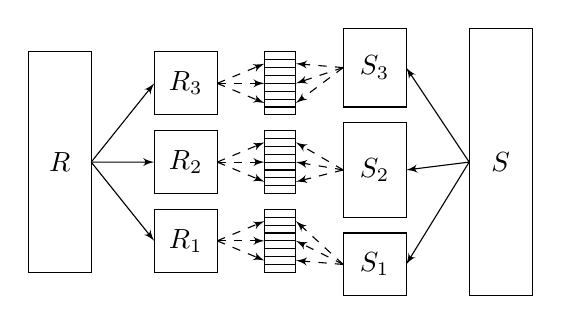
\begin{tikzpicture}[>=latex']
	\draw (-3.2cm,1cm) rectangle (-2.4cm,3.8cm);
	\node () at (-2.8,2.4cm) {$R$};
	\draw (3.2cm,0.7cm) rectangle (2.4cm,4.1cm);
	\node () at (2.8,2.4cm) {$S$};
	\foreach \y/\c in {1/1.1,2/2.3,3/3.6} {
		\draw (-1.6cm,\y cm) rectangle (-0.8cm,\y cm+0.8cm);
		\node () at (-1.2cm,\y cm+0.4cm) {$R_\y$};
		\node () at (1.2cm,\c cm) {$S_\y$};
		\path [->] (-2.4cm,2.4cm) edge (-1.6cm,\y cm+0.4cm);
		\path [->] (2.4cm,2.4cm) edge (1.6cm,\c cm);
		\path [->,dashed] (-0.8cm,\y cm+0.4cm) edge (-0.2cm,\y cm+0.15cm);
		\path [->,dashed] (-0.8cm,\y cm+0.4cm) edge (-0.2cm,\y cm+0.4cm);
		\path [->,dashed] (-0.8cm,\y cm+0.4cm) edge (-0.2cm,\y cm+0.65cm);
		\path [->,dashed] (0.8cm,\c cm) edge (0.2cm,\y cm+0.15cm);
		\path [->,dashed] (0.8cm,\c cm) edge (0.2cm,\y cm+0.4cm);
		\path [->,dashed] (0.8cm,\c cm) edge (0.2cm,\y cm+0.65cm);
		\draw (-0.2cm,\y cm) rectangle (0.2cm,\y cm+0.8cm);
		\foreach \yy in {0.1,0.2,...,0.7} {
			\draw (-0.2cm,\y cm + \yy cm) -- (0.2cm,\y cm + \yy cm);
		}
	}
	\draw (0.8cm,0.7 cm) rectangle (1.6cm,1.5cm);
	\draw (0.8cm,1.7cm) rectangle (1.6cm,2.9cm);
	\draw (0.8cm,3.1cm) rectangle (1.6cm,4.1cm);
\end{tikzpicture}
\end{center}
\caption[Grace Hash Join]{Grace hash join.}
\label{fig_hashjoin}
\end{figure}

The \emph{grace hash join} algorithms divides the relations $R$ and $S$ into partitions $R_1,\ldots,R_n$ and $S_1,\ldots,S_n$, using a hasfunction $h$. For all $1 \leq i \leq n$, every tuple $r \in R_i$ can only match tuples $s \in S_i$. Thus a hashtable $H_i$ (with another hash function $h'$) is used to join the tuples in $R_i$ and $S_i$.

\begin{algorithm}
\caption*{\bf GraceHashJoin($R$,$S$,$\alpha$)}
\begin{algorithmic}
\FORALL{tuples $r \in R$}
	\STATE{add $r$ to $R_{h(r.\alpha)}$}
\ENDFOR
\FORALL{tuples $s \in S$}
	\STATE{add $s$ to $S_{h(s.\alpha)}$}
\ENDFOR
\FORALL{partitions $i \in \{1,\ldots,n\}$}
	\STATE{build hastable $H_i$ for $R_i$}
	\FORALL{tuples $s \in S_i$}
		\STATE{probe $H_i$ and output matching tuples}
	\ENDFOR
\ENDFOR
\end{algorithmic}
\end{algorithm}

\begin{note}
The smaller relation $R$ is partitioned in such a way that every partition $R_i$ fits into main memory. This avoids rescanning the entire relation $S$.
\end{note}


% ------------------------------------------------------------------------------------------------ %
% SORTING VS HASHING
% ------------------------------------------------------------------------------------------------ %


\subsubsection{Sorting vs Hashing}

Both techniques, sorting and hashing, can be used for joins, grou-by etc. They have the same asymptotic complexity (in IO and CPU). However, sorting is more robust, but hashing has a better average case.


% ------------------------------------------------------------------------------------------------ %
% ------------------------------------------------------------------------------------------------ %
% TRANSACTIONS
% ------------------------------------------------------------------------------------------------ %


\section{Transaction Processing}


% ------------------------------------------------------------------------------------------------ %
% TRANSACTIONS
% ------------------------------------------------------------------------------------------------ %


\subsection{Transactions}

A \emph{transaction} $T_i$ consists of the following elementary operations:
\begin{itemize}
\item $b_i$ to indicate the beginning of a transaction (BOT),
\item $r_i[x]$ to read from a data item $x$,
\item $w_i[x]$ to write to a data item $x$,
\item $a_i$ to perform an abort and
\item $c_i$ to perform a commit.
\end{itemize}
Each transaction starts with a (often implicit) begin of transaction $b_i$ and ends with either an abort $a_i$ or commit $c_i$.

The order of the operations in $T_i$ defines a partial order $<_i$.


% ------------------------------------------------------------------------------------------------ %
% PROPERTIES OF TRANSACTIONS
% ------------------------------------------------------------------------------------------------ %


\subsubsection{Properties of Transactions}

The following four properties of a transaction are known as the \emph{ACID principle}:

\begin{itemize}
\item \emph{Atomicity:} A transaction is executed in its entirety or not at all.
\item \emph{Consistency:} A transaction executed in its entirety over a consistent database produces a consistent database.
\item \emph{Isolation:} A transaction executes as if it were alone in the system, regardless of other transactions.
\item \emph{Durability:} Commited changes of a transaction are never lost; i.e. they can be recovered after a system failure.
\end{itemize}


% ------------------------------------------------------------------------------------------------ %
% SAVEPOINTS AND BACKUPS
% ------------------------------------------------------------------------------------------------ %


\subsubsection{Savepoints and Backups}

Defining a \emph{savepoint} establishes a recoverable intermediate state. A \emph{backup} transaction resets the state of the database to the most recent savepoint.


% ------------------------------------------------------------------------------------------------ %
% CONFLICTING OPERATIONS
% ------------------------------------------------------------------------------------------------ %


\subsubsection{Conflicting Operations}

Two operations are \emph{conflicting} if uncontrolled cuncurrency causes potential inconcistency.
Consider the possible operations of two transactions $T_i$ and $T_j$ that acces the same data item $A$:
\begin{itemize}
\item $r_i[x]$ and $r_j[x]$ are not conflicting, because both operations do not modify the database. Thus their order is irrelevant.
\item $r_i[x]$ and $w_j[x]$ are conflicting, because, depending on their order $T_i$, is either reading the new or the old value.
\item $w_i[x]$ and $r_j[x]$ is analogous to the previous case.
\item $w_i[x]$ and $w_j[x]$ are conflicting, because the final state of the database depends on their order.
\end{itemize}


% ------------------------------------------------------------------------------------------------ %
% CONCURRENCY CONTROL THEORY
% ------------------------------------------------------------------------------------------------ %


\subsection{Cuncurrency Control Theory}


% ------------------------------------------------------------------------------------------------ %
% HISTORIES
% ------------------------------------------------------------------------------------------------ %


\subsubsection{Histories}

A \emph{history} $H$ for a set of transactions $\{T_1,\ldots,T_n\}$ is a sequence of operations with a partial order $<_H$, such that:
\begin{itemize}
\item $H$ contains all operations of every transaction $T_i$, i.e. $H = \bigcup_{i=1}^n T_i$
\item $<_H$ is compatible with all $<_i$, i.e $\left(\bigcup_{i=1}^n <_i\right) \subseteq <_H$.
\item If $p,q \in H$ are conflicting operations, then either $p <_H q$ or $q <_H p$ holds.
\end{itemize}

\begin{figure}[htbp]
\begin{center}
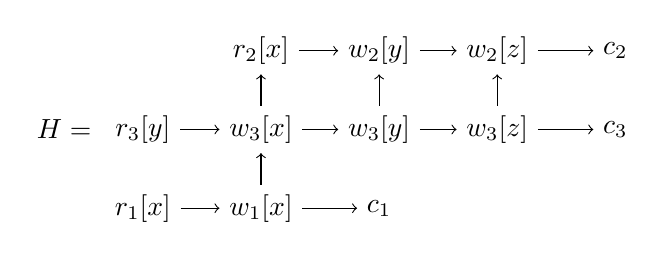
\begin{tikzpicture}
	\node (c2) at (1.5cm,2.0cm) {$r_2[x]$};
	\node (c3) at (3.0cm,2.0cm) {$w_2[y]$};
	\node (c4) at (4.5cm,2.0cm) {$w_2[z]$};
	\node (c5) at (6.0cm,2.0cm) {$c_2$};
	\node () at (-1.0cm,1.0cm) {$H=$};
	\node (b1) at (0.0cm,1.0cm) {$r_3[y]$};
	\node (b2) at (1.5cm,1.0cm) {$w_3[x]$};
	\node (b3) at (3.0cm,1.0cm) {$w_3[y]$};
	\node (b4) at (4.5cm,1.0cm) {$w_3[z]$};
	\node (b5) at (6.0cm,1.0cm) {$c_3$};
	\node (a1) at (0.0cm,0.0cm) {$r_1[x]$};
	\node (a2) at (1.5cm,0.0cm) {$w_1[x]$};
	\node (a3) at (3.0cm,0.0cm) {$c_1$};
	\path [->] (c2) edge (c3);
	\path [->] (c3) edge (c4);
	\path [->] (c4) edge (c5);
	
	\path [->] (b2) edge (c2);
	\path [->] (b3) edge (c3);
	\path [->] (b4) edge (c4);
	
	\path [->] (b1) edge (b2);
	\path [->] (b2) edge (b3);
	\path [->] (b3) edge (b4);
	\path [->] (b4) edge (b5);
	
	\path [->] (a2) edge (b2);
	
	\path [->] (a1) edge (a2);
	\path [->] (a2) edge (a3);
\end{tikzpicture}
\end{center}
\caption[Transaction History]{A history for three transactions.}
\label{fig_history}
\end{figure}

A history $H$ is \emph{serial}, if for every two transactions $T_i$ and $T_j$ in $H$, either all operations from $T_i$ appear before all operations of $T_j$ or vice versa.


% ------------------------------------------------------------------------------------------------ %
% EQUIVALENT HISTORIES
% ------------------------------------------------------------------------------------------------ %


\subsubsection{Equivalent Histories}

Two histories $H_1$ and $H_2$ are equivalent, if and only if
\begin{itemize}
\item they are over the same transactions and contain the same operations and
\item conflicting operations $p_i$ and $p_j$ of non aborted transactions are ordered in the same way in both histories, i.e $p_i <_{H_1} p_j$ holds if and only if $p_i <_{H_2} p_j$.
\end{itemize}


% ------------------------------------------------------------------------------------------------ %
% SERIALIZABLE HISTORY
% ------------------------------------------------------------------------------------------------ %


\subsubsection{Serializable History}

A history $H$ is \emph{serializable} if and only if it is equivalent to a serial history $H_s$. 

The \emph{serializability graph} $\msf{SG}(H)$ of a history $H$ over the transactions $T_1,\ldots,T_n$ is a compact representation of the dependencies in $H$. For every pair of conflicting operations $p_i$ and $q_j$ in $H$ with $p_i <_H q_j$, the edge $(T_i,T_j)$ is added to the serializability graph $\msf{SG}(H)$.

The \emph{serializability theorem} states that a history is serializable if and only if its serializability graph $\msf{SG}(H)$ is acyclic. A topological sort of $\msf{SG}(H)$ is a serial history $H_s$ with $H \equiv H_s$.

\begin{example}
	The serializability graph $\msf{SG}(H)$ of the history $H$ depicted in figure \ref{fig_history} is:
	\begin{center}
	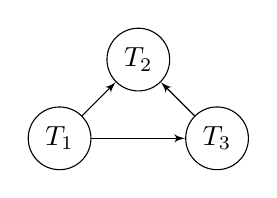
\begin{tikzpicture}[>=latex']
		\node [draw, circle] (t2) at (1cm,1cm) {$T_2$};
		\node [draw, circle] (t1) at (0cm,0cm) {$T_1$};
		\node [draw, circle] (t3) at (2cm,0cm) {$T_3$};
		\path [->] (t1) edge (t3);
		\path [->] (t1) edge (t2);
		\path [->] (t3) edge (t2);
	\end{tikzpicture}
	\end{center}
	Thus the history $H_s = T_1 \mid T_3 \mid T_2$ is serial and equivalent to the history $H$.
\end{example}


% ------------------------------------------------------------------------------------------------ %
% RECOVERY
% ------------------------------------------------------------------------------------------------ %


\subsection{Recovery Theory}


% ------------------------------------------------------------------------------------------------ %
% RECOVERABLE HISTORIES
% ------------------------------------------------------------------------------------------------ %


\subsubsection{Recoverable Histories}

In a history $H$, a transaction $T_i$ is said to \emph{reads} from another transaction $T_j$ if
\begin{itemize}
\item $T_i$ reads a data item $x$ that was written by $T_j$, i.e there are $r_i$ and $w_j$ with $w_j[x] <_H r_i[x]$,
\item $T_j$ does not abort before the read, i.e. $a_j \not<_H r_i[x]$ and
\item if there is a write $w_k[x]$ of another transaction with $w_j[x] <_H w_k[x] <_H r_i[x]$, then there is an $a_k <_H r_i[x]$.
\end{itemize}

A history $H$ is \emph{recoverable} if for every transaction $T_i$ reads from another transaction $T_j$ the condition $c_j <_H c_i$ holds. An abort in a recoverable history does not affect already commited transactions.


% ------------------------------------------------------------------------------------------------ %
% AVOIDING CASCADING ABORTS
% ------------------------------------------------------------------------------------------------ %


\subsubsection{Avoiding Cascading Aborts}

A history $H$ \emph{avoids cascading aborts (ACA)} if all transactions $T_i$ read only from committed transactions $T_j$, i.e $c_j <_H r_i[x]$.


% ------------------------------------------------------------------------------------------------ %
% STRICT HISTORIES
% ------------------------------------------------------------------------------------------------ %


\subsubsection{Strict Histories}

A history $H$ is \emph{strict} if for all $w_j[x] <_H p_i[x]$, where $p_i$ is a read or write operation, either $a_j <_H p_i[x]$ or $c_j <_H p_i[x]$ holds.


% ------------------------------------------------------------------------------------------------ %

\begin{figure}[htb]
\begin{center}
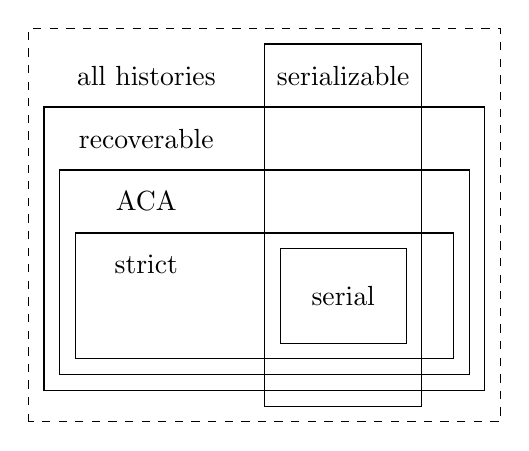
\begin{tikzpicture}
 	\path[area, dashed] (0.0cm,0.0cm) rectangle (6.0cm,5.0cm) {};
 	\path[area] (0.2cm,0.4cm) rectangle (5.8cm,4.0cm) {};
 	\path[area] (0.4cm,0.6cm) rectangle (5.6cm,3.2cm) {};
 	\path[area] (0.6cm,0.8cm) rectangle (5.4cm,2.4cm) {};
 	\path[area] (3.2cm,1.0cm) rectangle (4.8cm,2.2cm) {};
 	\path[area] (3.0cm,0.2cm) rectangle (5.0cm,4.8cm) {};
 	\node () at (1.5cm,4.4cm) {all histories};
 	\node () at (4.0cm,4.4cm) {serializable};
 	\node () at (1.5cm,3.6cm) {recoverable};
 	\node () at (1.5cm,2.8cm) {ACA};
 	\node () at (1.5cm,2.0cm) {strict};
 	\node () at (4.0cm,1.6cm) {serial};
\end{tikzpicture}
\end{center}
\caption[Classes of Histories]{Classes of histories.}
\end{figure}


% ------------------------------------------------------------------------------------------------ %
% DATABASE SCHEDULER
% ------------------------------------------------------------------------------------------------ %


\subsection{Database Scheduler}

The task of a \emph{database scheduler} is to order the operations of transactions $T_1,\ldots,T_n$ in such a way that the resulting history is reasonable. Serializability is often the minimal requirement. In general avoidance of cascading aborts is also required.


% ------------------------------------------------------------------------------------------------ %
% LOCK BASED SYNCHRONIZATION
% ------------------------------------------------------------------------------------------------ %


\subsection{Lock Based Synchronization}

Lock based synchronization is a widely used technique for schedulers. There are two sorts of locks:
\begin{itemize}
\item A \emph{schared lock} $S$ is acquired if a transaction wants to read from an object.
\item An \emph{exclusive lock} $X$ is acquired if a transaction wants to write to an object.
\end{itemize}


% ------------------------------------------------------------------------------------------------ %
% TWO PHASE LOCKING PROTOCOL
% ------------------------------------------------------------------------------------------------ %


\subsubsection{Two-Phase Locking Protocol}

The scheduler realizes serializability by following the \emph{two-phase locking  (2PL)} protocol. The following conditions must hold:
\begin{enumerate}
\item Every transaction must acquire a lock before accessing an object.
\item A transaction acquires a lock only once. Lock upgrades are possible.
\item A transaction is blocked if the lock requested cannot be granted.
\item Every transaction goes through two phases
	\begin{enumerate}
	\item Growth: Acquire locks, but never release a lock.
	\item Schrink: Release locks, but never acquire a lock.
	\end{enumerate}
\item At the end of a transaction (commit or abort) all locks must be released.
\end{enumerate}

\begin{figure}[htbp]
\begin{center}
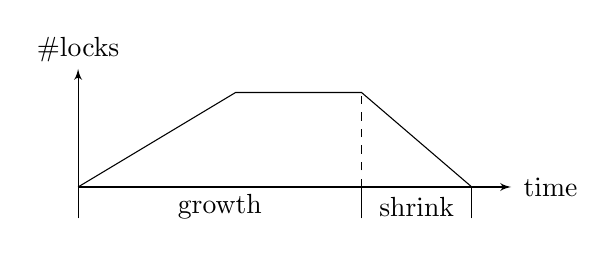
\begin{tikzpicture}[>=latex']
\node () at (0,1.75) {{\#}locks};
\node () at (1.8,-0.25) {growth};
\node () at (4.3,-0.25) {shrink};
\node () at (6,0) {time};
\draw [->] (0,0) -- (5.5,0);
\draw [->] (0,-0.4) -- (0,1.5);
\draw (3.6,-0.4) -- (3.6,0);
\draw [dashed] (3.6,0) -- (3.6,1.2);
\draw (5,-0.4) -- (5,0);
\draw (0,0) -- (2,1.2) -- (3.6,1.2) -- (5,0);
\end{tikzpicture}
\end{center}
\caption[Two-Phase Locking Protocol]{Visualization of the two-phase locking protocol.}
\end{figure}


% ------------------------------------------------------------------------------------------------ %
% STRICT TWO PHASE LOCKING PROTOCOL
% ------------------------------------------------------------------------------------------------ %


\subsubsection{Strict Two-Phase Locking Protocol}

The \emph{strict two-phase locking protocol} is like 2PL, except there is no shrink phase, i.e. all locks are kept until the end of the transaction.

\begin{figure}[htbp]
\begin{center}
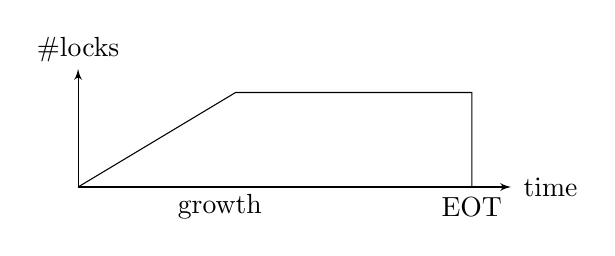
\begin{tikzpicture}[>=latex']
\node () at (0,1.75) {{\#}locks};
\node () at (1.8,-0.25) {growth};
\node () at (5,-0.25) {EOT};
\node () at (6,0) {time};
\draw [->] (0,0) -- (5.5,0);
\draw [->] (0,0) -- (0,1.5);
\draw (0,0) -- (2,1.2) -- (5,1.2) -- (5,0);
\end{tikzpicture}
\end{center}
\caption[Strict Two-Phase Locking Protocol]{Strict two-phase locking protocol.}
\end{figure}

\begin{note}
Strict 2PL avoids cascading aborts.
\end{note}

\todo (discussion of 2PL/ S2PL)


% ------------------------------------------------------------------------------------------------ %
% DEADLOCK DETECTION
% ------------------------------------------------------------------------------------------------ %


\subsubsection{Deadlock Detection}

A precise, but expensive, way to detect \emph{deadlocks} is the \emph{wait-for graph}: For every transaction $T_i$ that waits for another transaction $T_j$, the edge $(T_i,T_j)$ is added to the graph. There is a deadlock if and only if the wait-for graph has a cycle.

\begin{example}
A wait for-graph is depicted in figure \ref{fig_waitfor}. Aborting transaction $T_2$ or $T_3$ resolves both cycles.
\end{example}

\begin{figure}[htbp]
\begin{center}
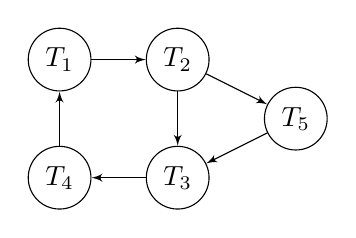
\begin{tikzpicture}[>=latex']
	\node [draw, circle] (n1) at (0,1.5) {$T_1$};
	\node [draw, circle] (n2) at (1.5,1.5) {$T_2$};
	\node [draw, circle] (n5) at (3,0.75) {$T_5$};
	\node [draw, circle] (n4) at (0,0) {$T_4$};
	\node [draw, circle] (n3) at (1.5,0) {$T_3$};
	\path [->] (n1) edge (n2);
	\path [->] (n2) edge (n3);
	\path [->] (n3) edge (n4);
	\path [->] (n4) edge (n1);
	\path [->] (n2) edge (n5);
	\path [->] (n5) edge (n3);
\end{tikzpicture}
\end{center}
\caption[Wait-For Graph]{Wait-for graph with two cycles.}
\label{fig_waitfor}
\end{figure}

Another way to detect deadlocks is to set a \emph{timeout} for every transaction's progress. If a timeout occurs, the system assumes a deadlock and resets the affected transaction.

A too short timeout leads to transactions being unnecessarily resetted, whereas a long timeout leads to prolonged deadlock situations.


% ------------------------------------------------------------------------------------------------ %
% SNAPSHOT ISOLATION
% ------------------------------------------------------------------------------------------------ %


\subsection{Snapshot Isolation}

In transaction processing, \emph{snapshot isolation (SI)} is a guarantee that all reads made in a transaction will see a consistent snapshot of the database:
\begin{enumerate}
\item When a transaction $T_i$ starts, it receives a timestamp $\tau_i$.
\item All reads are carried out as of the database at time $\tau_i$. Historic versions of all objects are needed.
\item All writes are carried out in a separate buffer and become visible after a commit.
\item When a transaction $T_i$ with timestamp $\tau_i$ commits, the DBMS checks for conflicts and aborts $T_i$ if there is another transaction $T_j$ with timestamp $\tau_j$ that updated the same object and $\tau_i < c_j < c_i$.
\end{enumerate}


\subsubsection{Lost Updates}

Figure \ref{fig_lost_update} shows two histories that are accepted by snapshot isolation, but the update of transaction $T_2$ is lost.

\begin{figure}[htbp]
\begin{center}
\begin{tabular}{|c|c|c|}\hline
  &  $T_1$   & $T_2$    \\\hline\hline
1 &          & $b_2$    \\
2 &          & $r_2[x]$ \\
3 & $b_1$    &          \\
4 & $r_1[x]$ &          \\
5 &          & $w_2[x]$ \\
6 &          & $c_2$    \\
7 & $w_1[x]$ &          \\
8 & $c_1$    &          \\\hline
\end{tabular}
\hspace{1em}
\begin{tabular}{|c|c|c|}\hline
  &  $T_1$   & $T_2$    \\\hline\hline
1 & $b_1$    &          \\
2 & $r_1[x]$ &          \\
3 &          & $b_2$    \\
4 &          & $r_2[x]$ \\
5 &          & $w_2[x]$ \\
6 &          & $c_2$    \\
7 & $w_1[x]$ &          \\
8 & $c_1$    &          \\\hline
\end{tabular}
\end{center}
\caption[Snapshot Isolation and Lost Update]{Snapshot isolation and lost update.}
\label{fig_lost_update}
\end{figure}

\subsubsection{Write Skew Anomaly}

In a \emph{write skew} anomaly, two transactions $T_1$ and $T_2$ concurrently read an overlapping data set (e.g. $x$ and $y$), concurrently make disjoint updates (e.g. $T_1$ updates $x$ and $T_2$ updates $y$, and finally commit, neither having seen the update performed by the other. In a serializable system, such an anomaly would be impossible.


\subsubsection{Comparison with Two-Phase Locking}

The history shown in figure \ref{fig_interesting} is accepted by both 2PL and SI. 2PL supports the serialization $T_2 \ra T_3 \ra T_1$ whereas SI enforces the serialization $T_1 \ra T_2 \ra T_3$, which may lead to inconsistency.

\begin{figure}[htbp]
\begin{center}
\begin{tabular}{|c|c|c|c|}\hline
   & $T_1$    & $T_2$    & $T_3$    \\\hline\hline
1  & $b_1$    &          &          \\
2  &          & $b_2$    &          \\
3  &          & $w_2[x]$ &          \\
4  &          & $w_2[y]$ &          \\
5  &          & $c_2$    &          \\
6  & $r_1[x]$ &          &          \\
7  &          &          & $b_3$    \\
8  &          &          & $r_3[z]$ \\
9  &          &          & $r_3[y]$ \\
10 &          &          & $c_3$    \\
11 & $w_1[z]$ &          &          \\
12 & $c_1$    &          &          \\\hline
\end{tabular}
\end{center}
\caption[Interesting History]{Interesting history.}
\label{fig_interesting}
\end{figure}

\begin{itemize}
\item \textbf{Two-phase locking:} A lock for every read or write is needed. There is a total order of conflicting operations. Operations are not re-ordered and only serializable histories are allowed.
\item \textbf{Snapshot isolation:} No read or write of a transaction is ever blocked; blocking only happens when a transaction commits. Aborts can be implemented very efficiently. There are no deadlocks, but unnecessary rollbacks. Non-serializable histories are allowed. Read-write conflicting operations are re-ordered and an abort is needed to deal with write-write conflicts.
\end{itemize}


% ------------------------------------------------------------------------------------------------ %
% DISTRIBUTED TRANSACTION PROCESSING
% ------------------------------------------------------------------------------------------------ %


\subsection{Distributed Transaction Processing}


% ------------------------------------------------------------------------------------------------ %
% ATOMIC COMMIT
% ------------------------------------------------------------------------------------------------ %


\subsubsection{Atomic Commit}

An \emph{atomic commit} enforces the following properties:
\begin{enumerate}
\item All processes that reach a decision reach the same one.
\item A process cannot reverse its decision.
\item A commit can only be decided if all processes vote yes.
\item If there are no failures and all processes voted yes, the decision will be to commit.
\item Consider an execution with normal failures. If all failures are repaired and no more failures occur for a sufficiently long time, then all processors will eventually reach a decision.
\end{enumerate}


% ------------------------------------------------------------------------------------------------ %
% TWO-PHASE COMMIT
% ------------------------------------------------------------------------------------------------ %


\subsubsection{Two-Phase Commit Protocol}

The \emph{two-phase commit protocol (2PC)} is a distributed algorithm that coordinates the processes that participate in a distributed atomic transaction on whether to commit or abort the transaction.

\begin{figure}[htbp]
\begin{center}
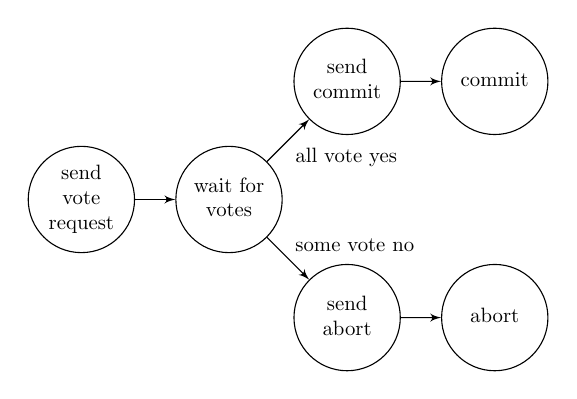
\begin{tikzpicture}[auto,>=latex',scale=\fsmscale]
	\fsmstate{s1}{0.0cm,0.0cm}{send\\ vote\\ request}
	\fsmstate{s2}{2.5cm,0.0cm}{wait for\\ votes}
	\fsmstate{s3}{4.5cm,2.0cm}{send\\ commit}
	\fsmstate{s4}{7.0cm,2.0cm}{commit}
	\fsmstate{s5}{4.5cm,-2.0cm}{send\\ abort}
	\fsmstate{s6}{7.0cm,-2.0cm}{abort}
	\draw [->] (s1) -- (s2);
	\draw [->] (s2) -- node [swap,scale=\fsmscale] {all vote yes} (s3);
	\draw [->] (s3) -- (s4);
	\draw [->] (s2) -- node [scale=\fsmscale] {some vote no} (s5);
	\draw [->] (s5) -- (s6);
\end{tikzpicture}
\end{center}
\caption[Two-Phase Commit Coordinator]{Two-phase commit coordinator.}
\label{fig_2pc_coordinator}
\end{figure}

\begin{figure}[htbp]
\begin{center}
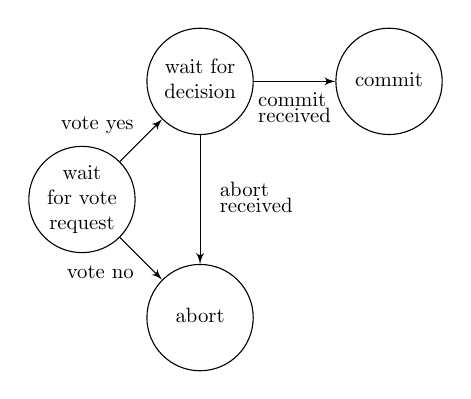
\begin{tikzpicture}[auto,>=latex',scale=\fsmscale]
	\fsmstate{s1}{0cm,0.0cm}{wait\\ for vote\\ request}
	\fsmstate{s2}{2.0cm,2.0cm}{wait for\\ decision}
	\fsmstate{s3}{5.2cm,2.0cm}{commit}
	\fsmstate{s4}{2.0cm,-2.0cm}{abort}
	\draw [->] (s1) -- node [scale=\fsmscale] {vote yes} (s2);
	\draw [->] (s2) -- node [swap,scale=\fsmscale] {\begin{tabular}{l}commit\\[-.4em] received\end{tabular}} (s3);
	\draw [->] (s1) -- node [swap,scale=\fsmscale] {vote no} (s4);
	\draw [->] (s2) -- node [scale=\fsmscale] {\begin{tabular}{l}abort\\[-.4em] received\end{tabular}} (s4);
\end{tikzpicture}
\end{center}
\caption[Two-Phase Commit Participant]{Two-phase commit participant.}
\label{fig_2pc_participant}
\end{figure}

\begin{enumerate}
\item The coordinator sends a \textit{vote request} to all participants.
\item Upon receiving a \textit{vote request}, a participant sends a message with yes or no. If the vote is no, the participant aborts the transaction and stops.
\item If the coordinator collects all votes and
	\begin{enumerate}
	\item sends \textit{commit} if all participants voted yes or
	\item sends \textit{abort} if there is a participant that voted no.
	\end{enumerate}
\item A participant that receives a \textit{commit} or \textit{receive} from the coordinator decides accordingly and stops.7
\end{enumerate}

If the coordinator times-out waiting fo votes, it can decide to abort. If a participant times-out waiting for a \textit{vote request}, it can decide to abort. But if a participant times-out waiting for a decision it cannot decide anything; this state is called uncertainty period.

When in doubt, ask if any process has decided yet. If the coordinator fails after receiving all votes but before sending any \textit{commit} message, all participants are uncertain and will not be able to decide anything until the coordinator recovers; they are blocked.

\begin{note}
2PC meets the five atomic commit conditions.
\end{note}


% ------------------------------------------------------------------------------------------------ %
% LINEAR TWO-PHASE COMMIT
% ------------------------------------------------------------------------------------------------ %


\subsubsection{Linear Two-Phase Commit Protocol}

The \emph{linear two-phase commit protocol} exploits a linear network topology to minimize the number of messages. The process $P_1$ starts the voting phase. If a process $P_i$ receives a \textit{yes} and wants to commit, it sends a \textit{yes} to process $P_{i+1}$. If the process $P_n$ receives a \textit{yes} and wants to commit, a \textit{commit} is sent back along all processes. If any process $P_i$ receives a \textit{yes} and wants to abort, it sends an \textit{abort} to $P_{i-1}$ and $P_{i+1}$. If a process receives an abort from one side, the abort is forwarded to the other side.

\begin{figure}[htbp]
\begin{center}
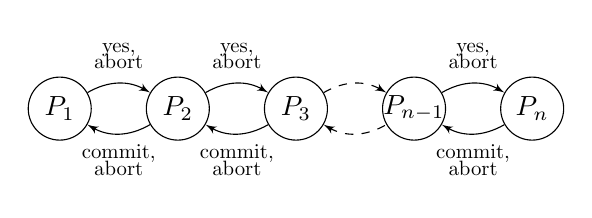
\begin{tikzpicture}[auto,>=latex']
\node [draw, circle, minimum width=0.8cm] (p1) at (0.0cm,0cm) {}; \node () at (0.0cm,0cm) {$P_1$};
\node [draw, circle, minimum width=0.8cm] (p2) at (1.5cm,0cm) {}; \node () at (1.5cm,0cm) {$P_2$};
\node [draw, circle, minimum width=0.8cm] (p3) at (3.0cm,0cm) {}; \node () at (3.0cm,0cm) {$P_3$};
\node [draw, circle, minimum width=0.8cm] (p4) at (4.5cm,0cm) {}; \node () at (4.5cm,0cm) {$P_{n-1}$};
\node [draw, circle, minimum width=0.8cm] (p5) at (6.0cm,0cm) {}; \node () at (6.00cm,0cm) {$P_n$};

\path [->] (p1) edge [bend left=] node [scale=\fsmscale] {\begin{tabular}{c}yes, \\[-.4em]abort\end{tabular}} (p2);
\path [->] (p2) edge [bend left] node [scale=\fsmscale] {\begin{tabular}{c}yes, \\[-.4em]abort\end{tabular}} (p3);
\path [->] (p4) edge [bend left] node [scale=\fsmscale] {\begin{tabular}{c}yes, \\[-.4em]abort\end{tabular}} (p5);
\path [<-] (p1) edge [bend right] node [scale=\fsmscale,swap] {\begin{tabular}{c}commit, \\[-.4em]abort\end{tabular}} (p2);
\path [<-] (p2) edge [bend right] node [scale=\fsmscale,swap] {\begin{tabular}{c}commit, \\[-.4em]abort\end{tabular}} (p3);
\path [<-] (p4) edge [bend right] node [scale=\fsmscale,swap] {\begin{tabular}{c}commit, \\[-.4em]abort\end{tabular}} (p5);
\path [->,dashed] (p3) edge [bend left] (p4);
\path [<-,dashed] (p3) edge [bend right] (p4);
\end{tikzpicture}
\end{center}
\caption[Linear Two-Phase Commit Protocol] {Message flow of the linear two-phase commit protocol.}
\label{fig_linear2pc}
\end{figure}

The total number of messages sent by linear 2PC is at most $2n$ instead of $3n$. But the number of rounds is $2n$ instead of only $3$.


% ------------------------------------------------------------------------------------------------ %
% THREE PHASE COMMIT
% ------------------------------------------------------------------------------------------------ %


\subsubsection{Three-Way Commit Protocol}

In the two-phase commit protocol there is the blocking situation in which all processes have voted yes but the coordinator fails. To avoid this situation the \emph{three-phase commit protocol (3PC)} enforces the non-blocking rule: \textit{No process can decide to commit if there are processes that are uncertain}.

\todo (WTF is this shit?)

\begin{figure}[htbp]
\begin{center}
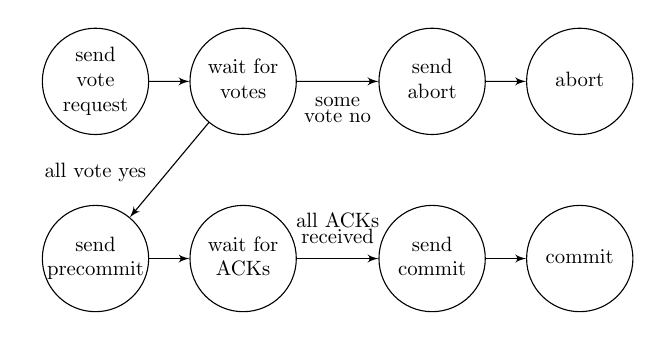
\begin{tikzpicture}[auto,>=latex',scale=\fsmscale]
	\fsmstate{s1}{0.0cm,3.0cm}{send \\vote \\request}
	\fsmstate{s2}{2.5cm,3.0cm}{wait for \\votes}
	\fsmstate{s3}{5.7cm,3.0cm}{send\\ abort}
	\fsmstate{s4}{8.2cm,3.0cm}{abort}
	\fsmstate{s5}{0.0cm,0.0cm}{send\\ precommit}
	\fsmstate{s6}{2.5cm,0.0cm}{wait for\\ ACKs}
	\fsmstate{s7}{5.7cm,0.0cm}{send\\ commit}
	\fsmstate{s8}{8.2cm,0.0cm}{commit}
	\draw [->] (s1) -- (s2);
	\draw [->] (s2) -- node [swap, scale=\fsmscale] {\begin{tabular}{c}some\\[-.4em] vote no\end{tabular}} (s3);
	\draw [->] (s3) -- (s4);
	\draw [->] (s2) -- node [swap, pos=0.7, scale=\fsmscale] {all vote yes} (s5);
	\draw [->] (s5) -- (s6);
	\draw [->] (s6) -- node [scale=\fsmscale] {\begin{tabular}{c}all ACKs\\[-.4em] received\end{tabular}} (s7);
	\draw [->] (s7) -- (s8);
\end{tikzpicture}
\end{center}
\caption[Three-Way Commit Coordinator]{Three-way commit coordinator.}
\end{figure}

\begin{figure}[htbp]
\begin{center}
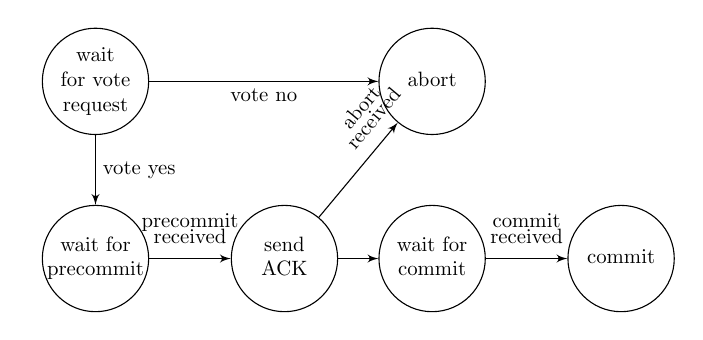
\begin{tikzpicture}[auto,>=latex',scale=\fsmscale]
	\fsmstate{s1}{0.0cm,3.0cm}{wait\\ for vote\\ request}
	\fsmstate{s2}{5.7cm,3.0cm}{abort}
	\fsmstate{s3}{0.0cm,0.0cm}{wait for\\ precommit}
	\fsmstate{s4}{3.2cm,0.0cm}{send\\ ACK}
	\fsmstate{s5}{5.7cm,0.0cm}{wait for\\ commit}
	\fsmstate{s6}{8.9cm,0.0cm}{commit}
	\draw [->] (s1) -- node [swap, scale=\fsmscale] {vote no} (s2);
	\draw [->] (s1) -- node [scale=\fsmscale] {vote yes} (s3);
	\draw [->] (s3) -- node [scale=\fsmscale] {\begin{tabular}{c}precommit\\[-.4em] received\end{tabular}} (s4);
	\draw [->] (s4) -- node [sloped, pos=0.9, scale=\fsmscale] {\begin{tabular}{c}abort\\[-.4em] received\end{tabular}} (s2);
	\draw [->] (s4) -- (s5);
	\draw [->] (s5) -- node [scale=\fsmscale] {\begin{tabular}{c}commit\\[-.4em] received\end{tabular}} (s6);
\end{tikzpicture}
\end{center}
\caption[Three-Way Commit Participant]{Three-way commit participant.\footnotemark}
\end{figure}

\footnotetext{This state diagram was copied from the lecture slides; but I cannot explain the transition from \textit{send ACK} to \textit{abort}.}


% ------------------------------------------------------------------------------------------------ %
% ------------------------------------------------------------------------------------------------ %
% REPLICATION
% ------------------------------------------------------------------------------------------------ %


\section{Replication}

Some reasons why \emph{replication} is used are:
\begin{itemize}
\item \textbf{Performance:} Location transparency is difficult to achieve in a distributed environment. If everything is local, all accesses should be fast.
\item \textbf{Fault tolerance:} If a site fails, the data it contains becomes unavailable. By keeping several copies, single site failures should not affect the overall availability.
\item \textbf{Application type:} To avoid interference, databases have always tried to seperate queries from updates.
\end{itemize}


% ------------------------------------------------------------------------------------------------ %
% REPLICATION STRATEGIES
% ------------------------------------------------------------------------------------------------ %


\subsection{Replication Strategies}

There are two basic parameters to select when designing a replication strategy.
\begin{itemize}
\item When to propagate the updates: synchronous (eager) or asynchronous (lazy).
\item Where the updates can take place: primary copy (master) or update everywhere (group).
\end{itemize}


% ------------------------------------------------------------------------------------------------ %
% SYNCHRONOUS
% ------------------------------------------------------------------------------------------------ %


\subsubsection{Synchronous Replication}

\emph{Synchronous replication} propagates any changes to the data immediately to all existing copies. Moreover, the changes are propagated within the scope of the transaction making the changes. The ACID properties apply to all copy updates.

\begin{itemize}
\item \textbf{Advantages:} There are no inconsistencies, i.e. all copies are identical. Thus reading the local copy yields the most up to date value. All changes are atomic.
\item \textbf{Disadvantages:} The execution time and response time are longer, because a transaction has to update all sites.
\end{itemize}


% ------------------------------------------------------------------------------------------------ %
% ASYNCHRONOUS
% ------------------------------------------------------------------------------------------------ %


\subsubsection{Asynchronous Replication}

\emph{Asynchronous replication} first executes the updating transaction on the local copy. Then the changes are propagated to all other copies. While the propagation takes place, the copies are inconsistent.

\begin{itemize}
\item \textbf{Advantages:} A transaction is always local, i.e. the response time is short.
\item \textbf{Disadvantages:} There are data inconsistencies. A local read does not always return te most up to date value. Changes to all copies are not guaranteed and the replication is not transparent.
\end{itemize}


% ------------------------------------------------------------------------------------------------ %
% UPDATE EVERYWHERE
% ------------------------------------------------------------------------------------------------ %


\subsubsection{Update Everywhere}

With an \emph{update everywhere} approach, changes can be initiated at any of the copies. That is, any of the sites which owns a copy can update the value of a data item.

\begin{itemize}
\item \textbf{Advantages:} Any site can run a transaction and the load is evenly distributed.
\item \textbf{Disadvantages:} All copies need to be synchronized.
\end{itemize}


% ------------------------------------------------------------------------------------------------ %
% PRIMARY COPY
% ------------------------------------------------------------------------------------------------ %


\subsubsection{Primary Copy}

With a \emph{primary copy} approach, there is only one copy which can be updated (the master), all others (secondary copies) are updated reflecting the changes to the master.


\begin{itemize}
\item \textbf{Advantages:} No inter-site synchronization is necessary; it takes place at the primary copy. There is always one site that has all the updates.
\item \textbf{Disadvantages:} The load at the primary copy can be quite large. Reading the local copy may not yield the most up to date value.
\end{itemize}


% ------------------------------------------------------------------------------------------------ %
% Replication Protocols
% ------------------------------------------------------------------------------------------------ %


\subsection{Replication Protocols}


% ------------------------------------------------------------------------------------------------ %
%


\subsubsection{Quorum Protocols}

\emph{Quorums}

\subsubsection{Deadlock Problem}

\subsubsection{Reconciliation}

\todo


% ------------------------------------------------------------------------------------------------ %
% ------------------------------------------------------------------------------------------------ %
% SECURITY
% ------------------------------------------------------------------------------------------------ %


\section{Database Security}


% ------------------------------------------------------------------------------------------------ %
% SECURITY TASKS
% ------------------------------------------------------------------------------------------------ %


\subsection{Security Tasks}

There are three kinds of security mechanisms in a DBMS:
\begin{itemize}
\item \emph{Authentication:} Verifying the identification of a user.
\item \emph{Authorization:} Checking the access privileges.
\item \emph{Auditing:} Looking for violations (in the past).
\end{itemize}
Data security consists of confidentality and integrity.


% ------------------------------------------------------------------------------------------------ %
% DISCRETIONARY ACCESS CONTROL
% ------------------------------------------------------------------------------------------------ %


\subsection{Discretionary Access Controls}

Access rules of \emph{discretionary acces controls (DAC)} assign access rights $t$ for an object $o$ to a subject $s$. Formally, access rules are quintuples $(o,s,t,p,f)$, where
\begin{itemize}
\item $o \in O$ and $O$ is the set of \emph{objects} (e.g. tables, tuples, attributes),
\item $s \in S$ and $S$ is the set of \emph{subjects} (e.g. users, processes, applications),
\item $t \in T$ and $T$ is the set of \emph{acces rights} (e.g. read, write, delete),
\item $p$ is a predicate (e.g. level = `c4') and
\item $f$ is a boolean value specifying, whether $s$ may grant the privilege $(o,t,p)$ to another subject $s' \in S$.
\end{itemize}

A simple way to store the access rules is a so called acces matrix. Other ways to control accesses are views or query rewriting.


% ------------------------------------------------------------------------------------------------ %
% ACCESS CONTRONL IN SQL
% ------------------------------------------------------------------------------------------------ %


\subsubsection{Access Control in SQL}


\begin{lstlisting}[language=sql,morekeywords={to}]
grant update (id, name, semester)
   on student
   to peter;
\end{lstlisting}

\begin{lstlisting}[language=sql,morekeywords={to}]
create view first_semester as
   select *
   from student
   where semester = 1;
grant select
   on first_semester
   to tutor;
\end{lstlisting}

Personal records can be protected by aggregation.

\clearpage



% ------------------------------------------------------------------------------------------------ %

\appendix

% ------------------------------------------------------------------------------------------------ %
% SQL
% ------------------------------------------------------------------------------------------------ %


\section{SQL}

The language \emph{SQL (Structured Query Language)} is designed for managing data in relational DMBS. It is based upon relational algebra and tuple relational calculus. SQL is a family of standards:

\begin{itemize}
\item Data definition language (DDL)
\item Data mnipulation language (DML)
\item Query Language
\end{itemize}

\begin{note}
In SQL relations are referred to as tables and may contain duplicates.
\end{note}


% ------------------------------------------------------------------------------------------------ %
% DATA TYPES
% ------------------------------------------------------------------------------------------------ %


\subsection{Data Types}

Some of SQL's data types are:
\begin{itemize}
\item \emph{char($n$):} strings of length $n$, padded with spaces.
\item \emph{varchar($n$):} strings of variable length with a maximum size of $n$ characters.
\item \emph{integer:} for interger values.
\item \emph{numeric($p$,$s$):} numbers with $p-s$ digits before the decimal and $s$ digits after the decimal.
\item \emph{blob, raw}: large binaries.
\item \emph{clob}: large string values.
\item \emph{date}: dates.
\end{itemize}


% ------------------------------------------------------------------------------------------------ %
% DATA DEFINITION LANGUAGE
% ------------------------------------------------------------------------------------------------ %


\subsection{Data Definition Language}

A \emph{data definition language (DDL)} is a syntax for defining or modifying data structures, especially database schemas. The following SQL statement illustrates, how a new table is created:
\begin{lstlisting}[language=sql]
create table student
  (id   integer     primary key,
   name varchar(20) not null),
   age  integer;
\end{lstlisting}

Columns of an existing table can be added and altered:
\begin{lstlisting}[language=sql]
alter table student
   add column semester integer;
alter table student
   alter column name varchar(30);
\end{lstlisting}

Similarly, a column is removed with \lstinline[language=sql]{drop column}. Indexes is created and deleted like this:

\begin{lstlisting}[language=sql]
create index my_index on
   student(name, age);
drop index my_index;
\end{lstlisting}


% ------------------------------------------------------------------------------------------------ %
% DATA MANIPULATION LANGUAGE
% ------------------------------------------------------------------------------------------------ %


\subsection{Data Manipulation Language}

A \emph{data manipulation language (DML)} is used to insert, update and delete tuples:
\begin{lstlisting}[language=sql]
insert into student (id, name)
   values (123, 'L. Skywalker');
update student
   set semester = semester+1;
delete student
   where age < 13;
\end{lstlisting}


% ------------------------------------------------------------------------------------------------ %
% QUERY
% ------------------------------------------------------------------------------------------------ %


\subsection{Queries}


\begin{lstlisting}[language=sql]
select [distinct] columns
   from tablename [as alias]
   [where condition]
   [group by (attribute)+]
   [having condition]
   [order by (attribute [asc|desc])+]
\end{lstlisting}

\begin{itemize}
\item The \emph{distinct} keywords eliminates all duplicate tuples.
\item Results are sorted using the \emph{order by} key words.
\end{itemize}

% ------------------------------------------------------------------------------------------------ %


\begin{center}
\begin{tabular}{|p{4em}|p{4em}|}\hline
$v$ & \bf not $v$ \\\hline
true       & false   \\
unknown    & unknown \\
false      & true    \\\hline
\end{tabular}
\end{center}

\begin{center}
\begin{tabular}{|p{4em}|p{4em}p{4em}p{4em}|}\hline
\bf and & true    & unknown & false   \\\hline
true    & true    & unknown & false   \\
unknown & unknown & unknown & false   \\
false   & false   & false   & false   \\\hline
\end{tabular}
\end{center}

\begin{center}
\begin{tabular}{|p{4em}|p{4em}p{4em}p{4em}|}\hline
\bf or  & true    & unknown & false   \\\hline
true    & true    & true    & true    \\
unknown & true    & unknown & unknown \\
false   & true    & unknown & false   \\\hline
\end{tabular}
\end{center}

% ------------------------------------------------------------------------------------------------ %


\subsection{Isolation in SQL92}

Isolation in a database determines how and when changes of a transaction becom visible for other transactions.

\begin{lstlisting}[morekeywords={set,transaction,isolation,level,diagnostic,size}]
set transaction
   [read only, | read write,]
   [isolation level
      read uncommited, |
      read commited,   |
      repeatable read, |
      serializable,]
   [diagnostic size ...,]
\end{lstlisting}

\begin{itemize}
\item \emph{Read uncommited:} This is the lowest level of isolation and is only allowed for read only transactions. Reads do not need a shared lock and are not hindered by exclusive locks.
\item \emph{Read commited:} Transactions only read commited versions of objects. However, one transaction may read different versions of an object.
\item \emph{Repeatable read} Reading different versions of the same object is prevented, but phantoms can still happen.
\item \emph{Serializable:} Full isolation is guaranteed.
\end{itemize}


% ------------------------------------------------------------------------------------------------ %
% integrity constriants

\label{LastPage}

\end{document}


% ------------------------------------------------------------------------------------------------ %